\documentclass[conference]{IEEEtran}
\IEEEoverridecommandlockouts
% The preceding line is only needed to identify funding in the first footnote. If that is unneeded, please comment it out.
\usepackage{amsmath,amssymb,amsfonts}
\usepackage{algorithmic}
\usepackage{graphicx}
\usepackage[inline, shortlabels]{enumitem}
\usepackage{tabularx}
\usepackage{caption}
\usepackage{titlesec}
\usepackage[T2A,T1]{fontenc}
\usepackage[english]{babel}
\captionsetup{font=it}
\usepackage{ragged2e}
\usepackage{hyperref}
\addto\extrasenglish{%
  \renewcommand{\sectionautorefname}{Section}%
  \renewcommand{\subsectionautorefname}{Subsection}%
  \renewcommand{\subsubsectionautorefname}{Subsubsection}%
  \renewcommand{\tableautorefname}{Table}%
  \renewcommand{\figureautorefname}{Figure}%
}
\usepackage{pifont}
\newcommand{\cmark}{\ding{51}}%
\newcommand{\xmark}{\ding{55}}%
\usepackage{footmisc}
\usepackage{multirow}

% --- Tickz
\usepackage{physics}
\usepackage{amsmath}
\usepackage{tikz}
\usepackage{mathdots}
\usepackage{yhmath}
\usepackage{float}
\usepackage{pdfpages}
\usepackage{stfloats}
\usepackage{cancel}
\usepackage{color}
\usepackage{siunitx}
\usepackage{array}
\usepackage{multirow}
\usepackage{amssymb}
\usepackage{gensymb}
\usepackage{tabularx}
\usepackage{extarrows}
\usepackage{booktabs}
\usetikzlibrary{fadings}
\usetikzlibrary{patterns}
\usetikzlibrary{shadows.blur}
\usetikzlibrary{shapes}

% ---------

\usepackage{pdfpages}
\usepackage{booktabs}
\usepackage{csquotes}
\usepackage{lipsum}  
\usepackage{arydshln}
\usepackage{smartdiagram}
\usepackage[inkscapeformat=png]{svg}
\usepackage{textcomp}
\usepackage{tabularray}\UseTblrLibrary{varwidth}
\usepackage{xcolor}
\def\BibTeX{{\rm B\kern-.05em{\sc i\kern-.025em b}\kern-.08em
    T\kern-.1667em\lower.7ex\hbox{E}\kern-.125emX}}
\usepackage{cite}
\usepackage{amsmath}
\newcommand{\probP}{\text{I\kern-0.15em P}}
\usepackage{etoolbox}
\patchcmd{\thebibliography}{\section*{\refname}}{}{}{}

\setlength{\extrarowheight}{2.5pt}

% \renewcommand{\arraystretch}{1.7}

% \setlength{\extrarowheight}{2.5pt}
% \renewcommand{\arraystretch}{0.2}
% \renewcommand{\arraystretch}{1.7}

% --------------
\titleclass{\subsubsubsection}{straight}[\subsection]

\newcounter{subsubsubsection}[subsubsection]
\renewcommand\thesubsubsubsection{\thesubsubsection.\arabic{subsubsubsection}}
\renewcommand\theparagraph{\thesubsubsubsection.\arabic{paragraph}} % optional; useful if paragraphs are to be numbered

\titleformat{\subsubsubsection}
  {\normalfont\normalsize\bfseries}{\thesubsubsubsection}{1em}{}
\titlespacing*{\subsubsubsection}
{0pt}{3.25ex plus 1ex minus .2ex}{1.5ex plus .2ex}

\makeatletter
\renewcommand\paragraph{\@startsection{paragraph}{5}{\z@}%
  {3.25ex \@plus1ex \@minus.2ex}%
  {-1em}%
  {\normalfont\normalsize\bfseries}}
\renewcommand\subparagraph{\@startsection{subparagraph}{6}{\parindent}%
  {3.25ex \@plus1ex \@minus .2ex}%
  {-1em}%
  {\normalfont\normalsize\bfseries}}
\def\toclevel@subsubsubsection{4}
\def\toclevel@paragraph{5}
\def\toclevel@paragraph{6}
\def\l@subsubsubsection{\@dottedtocline{4}{7em}{4em}}
\def\l@paragraph{\@dottedtocline{5}{10em}{5em}}
\def\l@subparagraph{\@dottedtocline{6}{14em}{6em}}
\makeatother

\setcounter{secnumdepth}{4}
\setcounter{tocdepth}{4}


\setboolean{@twoside}{false}

% --------------


\newcommand{\before}[1]{\textcolor{red}{#1}}
\newcommand{\after}[1]{\textcolor{green}{#1}}

\newcommand{\old}[1]{\textcolor{orange}{#1}}
\newcommand{\rem}[1]{\textcolor{red}{#1}}
\newcommand{\todo}[1]{\textcolor{orange}{\newline \textit{\textbf{TODO:} #1}} \newline \newline }

\makeatletter
\newcommand{\linebreakand}{%
  \end{@IEEEauthorhalign}
  \hfill\mbox{}\par
  \mbox{}\hfill\begin{@IEEEauthorhalign}
}
\makeatother




% ---------------------------


\begin{document}

\title{Streamlining Resilient Kubernetes Autoscaling with Multi-Agent Systems via an Automated Online Design Framework\\
    % {\footnotesize \textsuperscript{Note}}
    % \thanks{Identify applicable funding agency here. If none, delete this.}
}

% \IEEEaftertitletext{\vspace{-1\baselineskip}}

\author{

    \IEEEauthorblockN{Julien Soulé}
    \IEEEauthorblockA{\textit{Thales Land and Air Systems, BU IAS}}
    %Rennes, France \\
    \IEEEauthorblockA{\textit{Univ. Grenoble Alpes,} \\
        \textit{Grenoble INP, LCIS, 26000,}\\
        Valence, France \\
        julien.soule@lcis.grenoble-inp.fr}

    \and

    \IEEEauthorblockN{Jean-Paul Jamont\IEEEauthorrefmark{1}, Michel Occello\IEEEauthorrefmark{2}}
    \IEEEauthorblockA{\textit{Univ. Grenoble Alpes,} \\
        \textit{Grenoble INP, LCIS, 26000,}\\
        Valence, France \\
        \{\IEEEauthorrefmark{1}jean-paul.jamont,\IEEEauthorrefmark{2}michel.occello\}@lcis.grenoble-inp.fr
    }

    % \and

    % \IEEEauthorblockN{Michel Occello}
    % \IEEEauthorblockA{\textit{Univ. Grenoble Alpes,} \\
    % \textit{Grenoble INP, LCIS, 26000,}\\
    % Valence, France \\
    % michel.occello@lcis.grenoble-inp.fr}

    % \and

    \linebreakand

    \hspace{-0.5cm}
    \IEEEauthorblockN{Paul Théron}
    \IEEEauthorblockA{
        \hspace{-0.5cm}
        \textit{AICA IWG} \\
        \hspace{-0.5cm}
        La Guillermie, France \\
        \hspace{-0.5cm}
        %lieu-dit Le Bourg, France \\
        paul.theron@orange.fr}

    \and

    \hspace{0.5cm}
    \IEEEauthorblockN{Louis-Marie Traonouez}
    \IEEEauthorblockA{
        \hspace{0.5cm}
        \textit{Thales Land and Air Systems, BU IAS} \\
        \hspace{0.5cm}
        Rennes, France \\
        \hspace{0.5cm}
        louis-marie.traonouez@thalesgroup.com}}


\maketitle

\begin{abstract}
    In cloud-native systems, Kubernetes clusters with interdependent services often face challenges to their operational resilience due to poor workload management issues such as resource blocking, bottlenecks, or continuous pod crashes. These vulnerabilities are further amplified in adversarial scenarios, such as Distributed Denial-of-Service attacks. Conventional Horizontal Pod Autoscaling (HPA) approaches struggle to address such dynamic conditions, while reinforcement learning-based methods, though more adaptable, typically optimize single objectives like latency or resource usage, neglecting broader failure scenarios.
    %
    We propose decomposing the overarching objective of maintaining operational resilience into failure-specific sub-objectives delegated to collaborative agents, collectively forming an HPA Multi-Agent System (MAS). We introduce an automated, four-phase online framework for HPA MAS design: 1) modeling a digital twin built from cluster traces; 2) training agents in simulation using roles and missions tailored to failure contexts; 3) analyzing agent behaviors for explainability; and 4) transferring learned policies to the real cluster.
    %
    Experimental results demonstrate that the generated HPA MASs outperform three state-of-the-art HPA systems in sustaining operational resilience under various adversarial conditions in a proposed complex cluster.

\end{abstract}

\begin{IEEEkeywords}
    Adversarial, Horizontal Pod Autoscaling, Multi-Agent Reinforcement Learning, Multi-Agent System Design
\end{IEEEkeywords}

\section{Introduction}
\label{sec:introduction}

% Contexte
Cloud-native critical systems are increasingly reliant on Kubernetes to orchestrate and manage interdependent services~\cite{Pahl2019}. HPA is a widely adopted mechanism to dynamically adjust the number of pods based on resource usage, enabling systems to handle highly dynamic workloads~\cite{Hohpe2012}. However, failures such as pod crashes, resource contention, and bottlenecks can severely jeopardize the performance of all of the cluster's functionalities we globally refer to as operational resilience~\cite{Burns2016}. Worse, these failures may be exploited by attackers to degrade performance or induce outages, as seen in adversarial contexts like DDoS attacks~\cite{Koller2019}.

In such adversarial scenarios, malicious actors can exploit scaling mechanisms, exposing the limitations of conventional HPA systems~\cite{Kim2020}. Modern approaches have sought to address these gaps using Reinforcement Learning (RL), where an agent optimizes a single global objective such as minimizing latency or resource usage~\cite{Nguyen2019}. While these methods demonstrate adaptability, they often fall short in handling diverse failure scenarios to maintain \textit{Quality of Service} (QoS)~\cite{Castro2020}. For example, prioritizing responses to cascading pod crashes during an attack may be far more critical than reducing latency. These challenges highlight the need for an autoscaling system capable of dynamically balancing multiple sub-objectives to maintain all of the QoS to maximize operational resilience.

Achieving this shift from single-objective optimization to a multi-objective approach is complex~\cite{Shoham2008}. A single-agent RL system struggles to address such complexity due to the difficulty of coordinating responses to diverse and context-dependent failures~\cite{Jennings1998}. In contrast, Multi-Agent Systems (MASs) offer a promising paradigm by decomposing the overarching operational resilience maximization goal into sub-objectives handled by specialized agents~\cite{Shoham2008}. Considering an adversarial scenario, each defender agent can collaboratively contribute to complementary scaling actions towards reaching its own sub-objective, enabling more resilient and context-specific responses face to an attacker agent~\cite{Jennings1998}. We refer to the set of these collaborative agents as an HPA MAS. An HPA MAS actually builds upon the cyberdefense framework of Autonomous Intelligent Cybersecurity Agents (AICAs), which can be viewed as agents with specialized roles and missions collaboratively defending systems against attackers~\cite{Kott2018}.

% Problématique
However, designing HPA MASs tailored to a cluster presents significant challenges such as the need for detailed cluster knowledge, the time-consuming nature of manual design processes, and the difficulty of ensuring optimal agent behavior. Moreover, cluster changes require repeating the design process, increasing operational costs and complexity.

% Contribution
Among methdological works, we inspired from the \textit{Assisted MAS Organization Engineering Approach} (AOMEA)~\cite{soule2024aomea} that shows to align the most with automation and safety challenges. Based on AOMEA, we propose the \textit{Kubernetes Autoscaling with Resilient Multi-Agent system} (KARMA) to automate the design and implementation process through four sequential phases:
\begin{enumerate*}[label=\textbf{\arabic*)}, itemjoin={;\quad }]
    \item \textbf{Modeling}: Creating a digital twin of the cluster from real-world traces to simulate failure scenarios
    \item \textbf{Training}: Training agents in simulation using roles and missions that integrate explicit rule-based and guidance strategies
    \item \textbf{Analyzing}: Validating trained agents' behaviors and extracting design insights through empirical analysis
    \item \textbf{Transferring}: Running trained agents to apply their learned behaviors via the real Kubernetes API.
\end{enumerate*}

This framework enables to iteratively updates the simulation model with newly collected traces, enabling adaptation to cluster changes. We validated our approach on two adversarial scenarios from the "Chained Service" Kubernetes environment. The MASs were generated with minimal manual intervention, and demonstrate originality and robustness. They consistently outperformed state-of-the-art HPA systems, including AWARE~\cite{aware2023}, Gym-HPA~\cite{gymhpa2022}, IMAM~\cite{imam2022}, and Libra~\cite{Libra}, in maximizing operational resilience.

% Organisation
The remainder is structured as follows:
\autoref{sec:related_work} reviews existing HPA techniques and their limitations in dynamic environments.
\autoref{sec:proposed_approach} details our framework leveraging related concepts for each phase.
\autoref{sec:experiments} describes the experimental setup.
\autoref{sec:results} presents and discusses results.
\autoref{sec:conclusion} concludes and provides future directions.

% ===================================

\section{Related Work}
\label{sec:related_work}

\begin{table}[h!]
    \centering
    \caption{A KARMA overview regarding selected HPA Systems}
    \label{tab:autoscaling_criteria}
    {\scriptsize
    \renewcommand{\arraystretch}{1.1}
    % \resizebox{0.5\textwidth}{!}{%
    \begin{tabular}{>{\raggedright\arraybackslash}m{1.27cm}>{\centering\arraybackslash}m{0.47cm}>{\centering\arraybackslash}m{0.47cm}>{\centering\arraybackslash}m{0.47cm}>{\centering\arraybackslash}m{0.47cm}>{\centering\arraybackslash}m{0.47cm}>{\centering\arraybackslash}m{0.47cm}>{\centering\arraybackslash}m{0.47cm}>{\centering\arraybackslash}m{0.47cm}>{\centering\arraybackslash}m{0.75cm}}
    \hline
    \textbf{Criterion} & \vspace{-0.3cm}\textbf{\cite{gymhpa2022}} & \vspace{-0.3cm}\textbf{\cite{aware2023}} & \vspace{-0.3cm}\textbf{\cite{imam2022}} & \vspace{-0.3cm}\textbf{\cite{Libra}} & \vspace{-0.3cm}\textbf{\cite{QoSRL}} & \vspace{-0.3cm}\textbf{\cite{AHPA}} & \vspace{-0.3cm}\textbf{\cite{KOSMOS}} & \vspace{-0.3cm}\textbf{\cite{COPA}} \\
    \hline
    \hline
    Adversarial Scenarios & No & Partial & No & No & No & No & No & Partial \\
    \hline
    Multi-objective & No & Yes & Partial & Partial & Yes & No & Yes & No \\
    \hline
    Automation & High & Mid. & Mid. & Mid. & High & Mid. & Mid. & Mid. \\
    \hline
    Learning & Yes & Yes & Yes & Yes & Yes & No & No & No \\
    \hline
    Multi-Agent System & No & No & Yes & No & No & No & No & No \\
    \hline
    Simulation & Yes & No & Yes & Yes & Yes & No & No & No \\
    \hline
    Real env. & No & Yes & Yes & Yes & Yes & Yes & Yes & Yes \\
    \hline
    Explainable & No & No & No & No & No & No & No & No \\
    \hline
    Adaptation & High & Mid. & High & Mid. & Mid. & High & High & Mid. \\
    \hline
    Safety Guarantees & No & No & No & No & No & No & No & No \\
    \hline
    \end{tabular}%
    }
  \end{table}


Autoscaling in Kubernetes has traditionally relied on metrics-based approaches, such as the default Kubernetes Horizontal Pod Autoscaler (KHPA), which adjusts the number of pods based on CPU and memory utilization~\cite{KubernetesChallenges}. While effective for basic scaling, such methods fail to address dynamic or adversarial workloads, as they rely on reactive, threshold-based rules~\cite{AutoscalingLimitations}. To overcome these limitations, recent research has turned to Machine Learning (ML) and RL.

% \subsection*{Reinforcement Learning-Based Systems}
Four RL-based systems stand out for their innovative approaches, applicability, and relevance:
%
\begin{itemize}
    \item \textbf{Gym-HPA}~\cite{gymhpa2022} serves as a benchmark RL environment, enabling experimentation with various RL algorithms. It excels in adaptability to simulated workloads with a high degree of automation but lacks multi-objective support, explainability, and real-world applicability
    \item \textbf{AWARE}~\cite{aware2023} incorporates RL to optimize autoscaling decisions while balancing QoS objectives, such as response time and throughput. It partially considers adversarial scenarios but struggles with high automation levels and multi-agent coordination
    \item \textbf{IMAM}~\cite{imam2022} integrates RL with a multi-agent framework, making it highly adaptive in microservice-based architectures. However, it lacks safety guarantees and explainability, limiting its effectiveness in adversarial contexts
    \item \textbf{Libra}~\cite{Libra} introduces traffic-aware scaling in edge environments. While it provides valuable insights into traffic optimization, it lacks consideration for multi-objective trade-offs or safety-critical guarantees.
\end{itemize}

These systems highlight significant progress in RL-based autoscaling but share common limitations: a lack of comprehensive adversarial adaptability, limited support for multi-agent systems, and no explicit focus on explainability or safety guarantees.
%
% \subsection*{Hybrid and Rule-Based Approaches}
Other notable systems combine ML or rule-based strategies with traditional autoscaling:
%
\begin{enumerate*}[label={}, itemjoin={;\quad }]
    \item \textbf{QoS-Aware RL}~\cite{QoSRL} focuses on maintaining QoS under dynamic workloads but does not integrate seamlessly with Kubernetes-native features or consider adversarial scenarios
    \item \textbf{AHPA}~\cite{AHPA} and \textbf{KOSMOS}~\cite{KOSMOS} explore adaptive and combined vertical-horizontal scaling strategies, offering high adaptability but lacking learning capabilities
    \item \textbf{COPA}~\cite{COPA} emphasizes combined metrics-based autoscaling but remains reactive and limited in adversarial scenarios.
\end{enumerate*}

% \subsection*{Positioning Our Contribution}
KARMA addresses key gaps in \textbf{(1) operational resilience} for autoscaling by introducing an automated HPA MAS design framework. Unlike conventional approaches, which often fail under \textbf{(2) adversarial conditions}, KARMA decomposes maintaining operational resilience into failure-specific missions and roles, enabling agents to handle coordinate response to \textbf{bottlenecks}, \textbf{resource contention}, \textbf{DDoS}, and \textbf{pod crashes}. It combines \textbf{(3) digital twin modeling} with \textbf{(4) automated MAS generation} via Multi-Agent Reinforcement Learning (MARL) integrating \textbf{constraint satisfaction} to these roles and missions, streamlining HPA MAS design with minimal manual intervention. Leveraging this decomposition, KARMA seeks for a better \textbf{(5) adaptability} while also enabling a better \textbf{(6) explainability} as for decision making in the whole HPA MAS.


% ===================================
\section{KARMA: A framework for HPA MAS design and development}
\label{sec:proposed_approach}

This section overviews the KARMA framework to helps in designing a HPA MAS then details each one of its phase.

\subsection{KARMA Overview}

\begin{figure}[h!]
    \centering
    


\tikzset{every picture/.style={line width=0.75pt}} %set default line width to 0.75pt        

\begin{tikzpicture}[x=0.75pt,y=0.75pt,yscale=-1.2,xscale=1.2]
%uncomment if require: \path (0,1414); %set diagram left start at 0, and has height of 1414

%Straight Lines [id:da5609883377896374] 
\draw [color={rgb, 255:red, 74; green, 144; blue, 226 }  ,draw opacity=1 ][line width=2.25]    (317.22,111.13) -- (360.07,111.13) ;
\draw [shift={(365.07,111.13)}, rotate = 180] [fill={rgb, 255:red, 74; green, 144; blue, 226 }  ,fill opacity=1 ][line width=0.08]  [draw opacity=0] (5.72,-2.75) -- (0,0) -- (5.72,2.75) -- cycle    ;
%Image [id:dp9396292457736715] 
\draw (106.77,60.95) node  {
\includegraphics[width=18.66pt,height=18.36pt]{figures/karma_architecture/pod.png}};
%Image [id:dp3874378335758297] 
\draw (145.86,60.95) node  {
\includegraphics[width=18.66pt,height=18.36pt]{figures/karma_architecture/pod.png}};
%Shape: Rectangle [id:dp4562827234223257] 
\draw  [color={rgb, 255:red, 74; green, 144; blue, 226 }  ,draw opacity=1 ][line width=1.5]  (89,28.36) .. controls (89,25.6) and (91.24,23.36) .. (94,23.36) -- (255,23.36) .. controls (257.76,23.36) and (260,25.6) .. (260,28.36) -- (260,132) .. controls (260,134.76) and (257.76,137) .. (255,137) -- (94,137) .. controls (91.24,137) and (89,134.76) .. (89,132) -- cycle ;
%Image [id:dp9455935833751838] 
\draw (172.5,16.24) node  {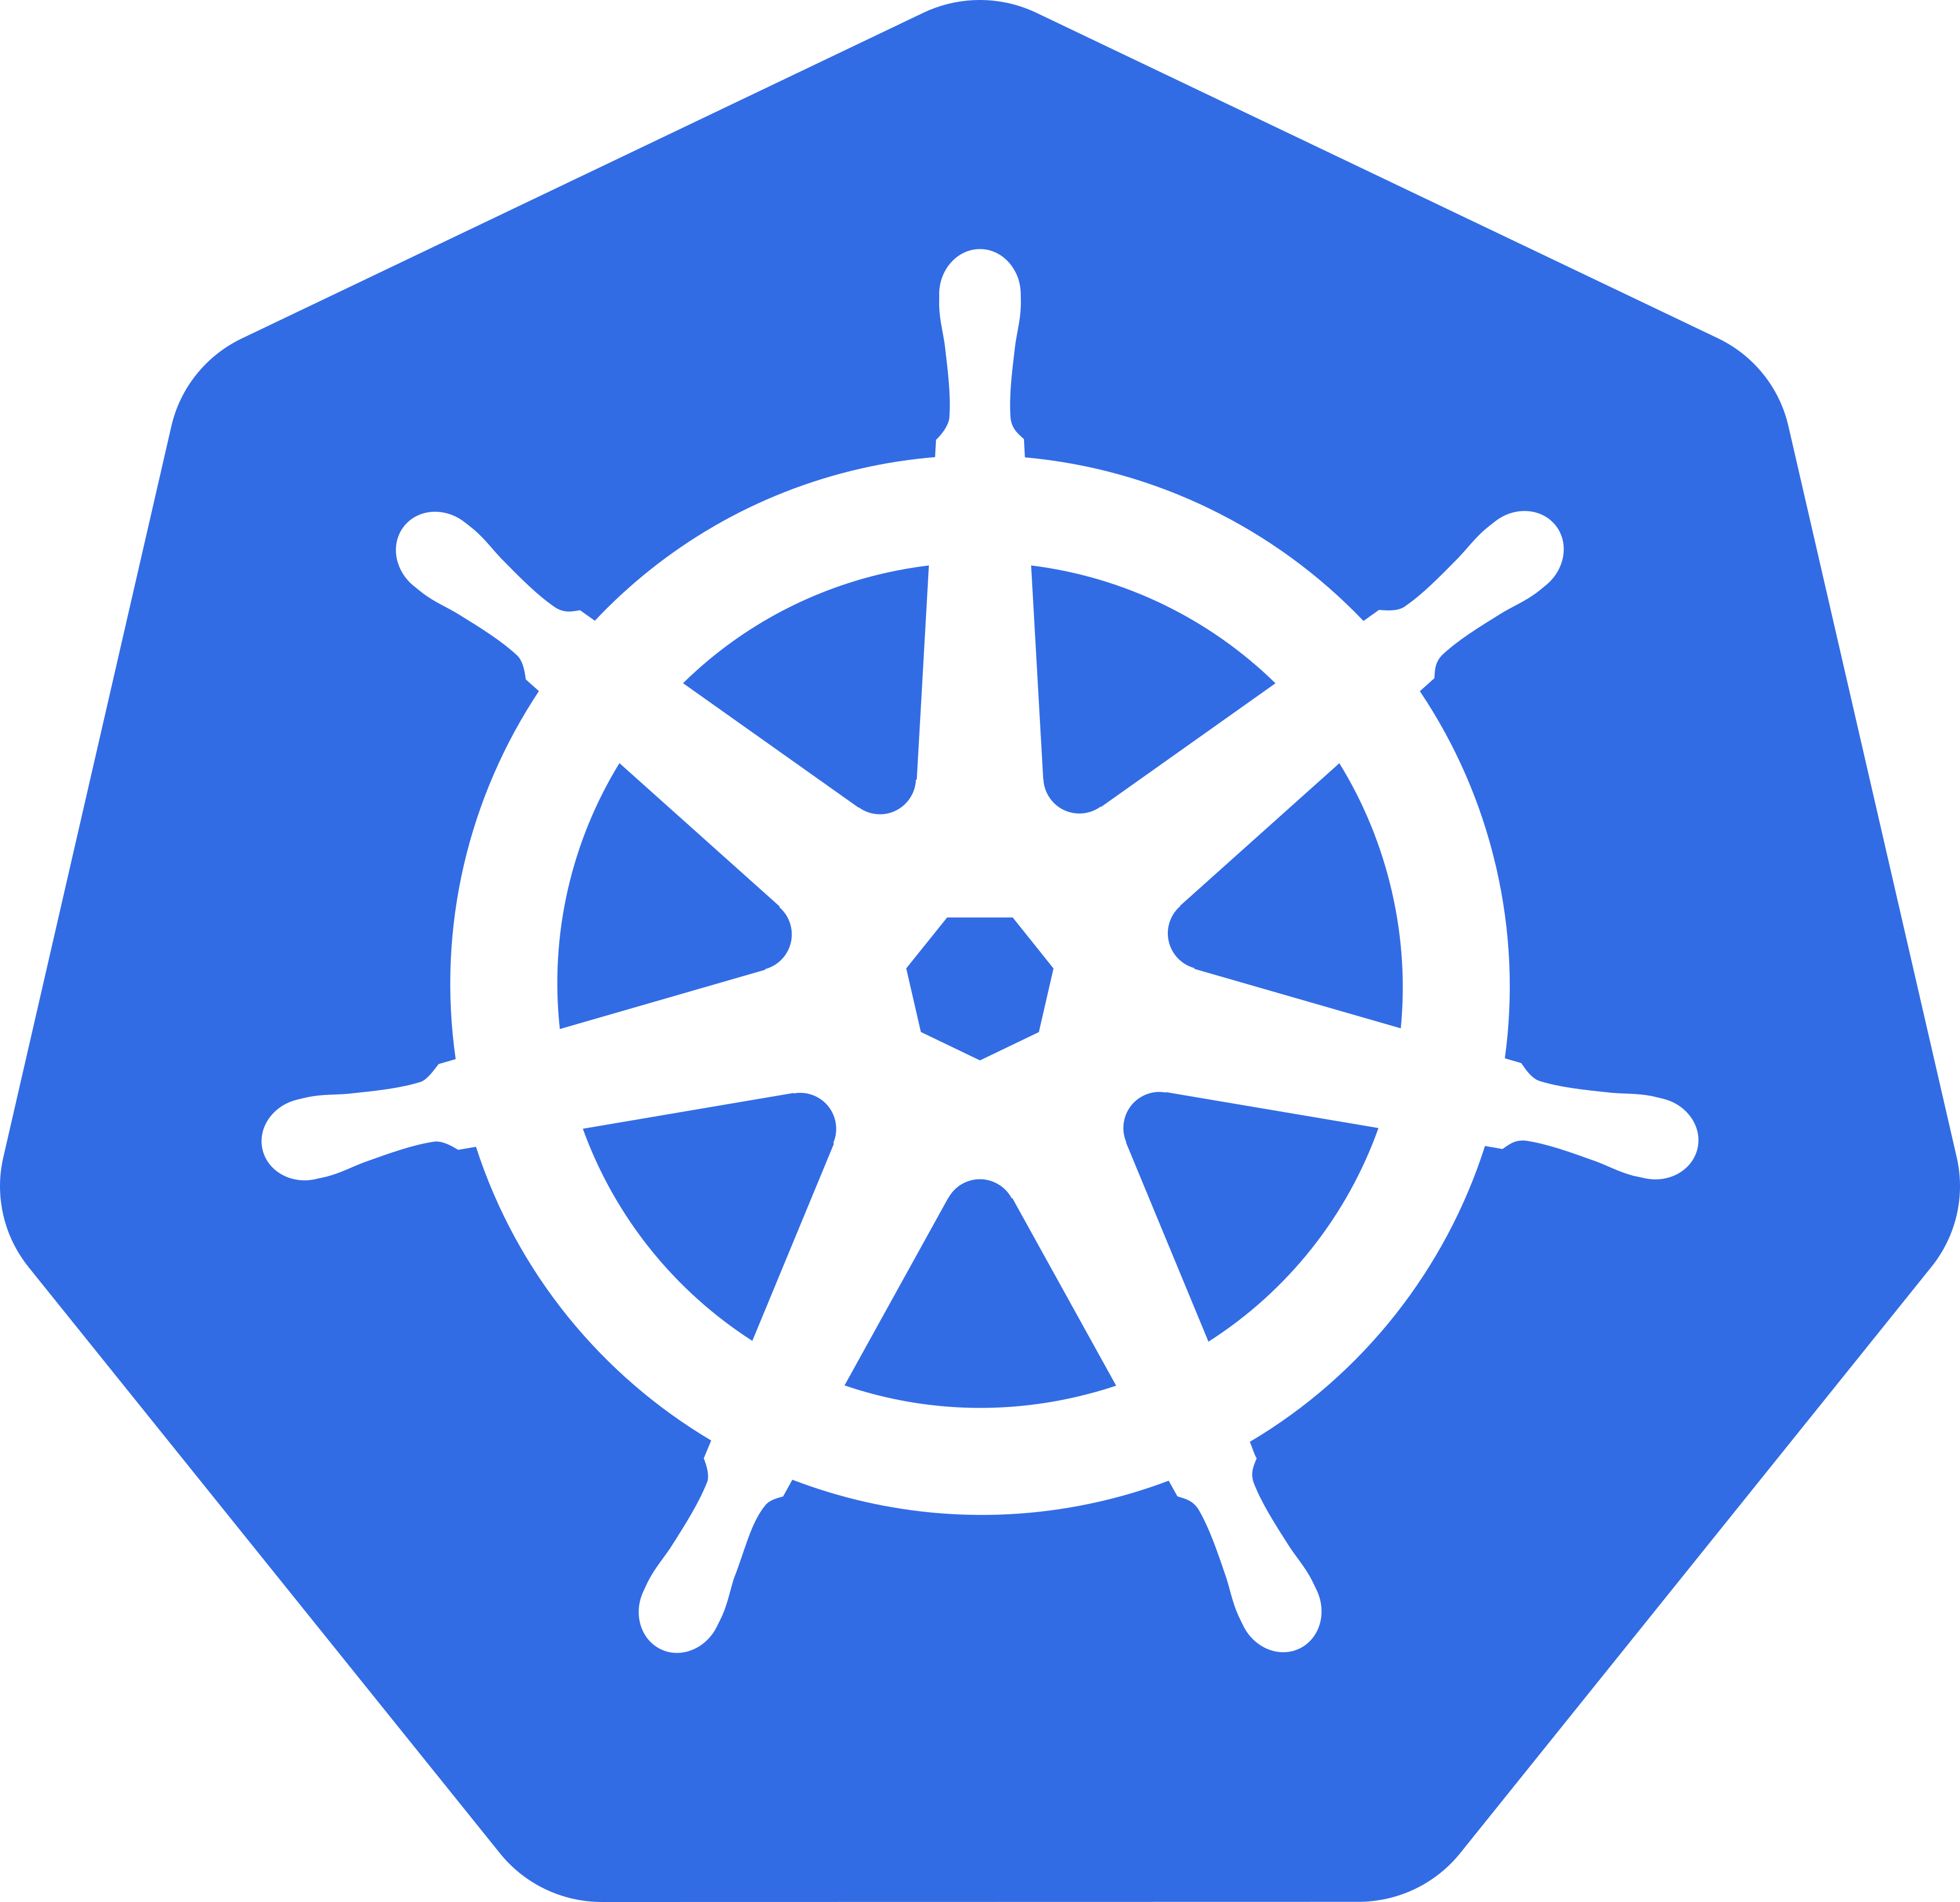
\includegraphics[width=18.66pt,height=18.36pt]{figures/karma_architecture/kubernetes.png}};
%Shape: Rectangle [id:dp9564725691593288] 
\draw  [color={rgb, 255:red, 74; green, 144; blue, 226 }  ,draw opacity=1 ][line width=1.5]  (92.55,50.21) .. controls (92.55,47.45) and (94.79,45.21) .. (97.55,45.21) -- (155.08,45.21) .. controls (157.84,45.21) and (160.08,47.45) .. (160.08,50.21) -- (160.08,70.81) .. controls (160.08,73.57) and (157.84,75.81) .. (155.08,75.81) -- (97.55,75.81) .. controls (94.79,75.81) and (92.55,73.57) .. (92.55,70.81) -- cycle ;
%Image [id:dp9120856447688912] 
\draw (126.32,39.97) node  {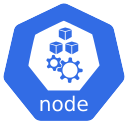
\includegraphics[width=18.66pt,height=18.36pt]{figures/karma_architecture/node.png}};
%Image [id:dp5738167237736518] 
\draw (106.77,119.52) node  {
\includegraphics[width=18.66pt,height=18.36pt]{figures/karma_architecture/pod.png}};
%Image [id:dp2199681121060142] 
\draw (145.86,119.52) node  {
\includegraphics[width=18.66pt,height=18.36pt]{figures/karma_architecture/pod.png}};
%Shape: Rectangle [id:dp12159705904547402] 
\draw  [color={rgb, 255:red, 74; green, 144; blue, 226 }  ,draw opacity=1 ][line width=1.5]  (92.55,108.78) .. controls (92.55,106.02) and (94.79,103.78) .. (97.55,103.78) -- (155.08,103.78) .. controls (157.84,103.78) and (160.08,106.02) .. (160.08,108.78) -- (160.08,129.38) .. controls (160.08,132.14) and (157.84,134.38) .. (155.08,134.38) -- (97.55,134.38) .. controls (94.79,134.38) and (92.55,132.14) .. (92.55,129.38) -- cycle ;
%Image [id:dp37768653229718074] 
\draw (126.32,98.54) node  {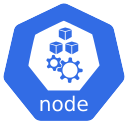
\includegraphics[width=18.66pt,height=18.36pt]{figures/karma_architecture/node.png}};
%Shape: Rectangle [id:dp20840815212238661] 
\draw  [color={rgb, 255:red, 74; green, 144; blue, 226 }  ,draw opacity=1 ][line width=1.5]  (264,28.36) .. controls (264,25.6) and (266.24,23.36) .. (269,23.36) -- (411.78,23.36) .. controls (414.54,23.36) and (416.78,25.6) .. (416.78,28.36) -- (416.78,132) .. controls (416.78,134.76) and (414.54,137) .. (411.78,137) -- (269,137) .. controls (266.24,137) and (264,134.76) .. (264,132) -- cycle ;
%Straight Lines [id:da9232180983272227] 
\draw [color={rgb, 255:red, 74; green, 144; blue, 226 }  ,draw opacity=1 ][line width=2.25]    (164,112) -- (201,112) ;
\draw [shift={(206,112)}, rotate = 180] [fill={rgb, 255:red, 74; green, 144; blue, 226 }  ,fill opacity=1 ][line width=0.08]  [draw opacity=0] (5.72,-2.75) -- (0,0) -- (5.72,2.75) -- cycle    ;
%Straight Lines [id:da6082715106712999] 
\draw [color={rgb, 255:red, 74; green, 144; blue, 226 }  ,draw opacity=1 ][line width=2.25]    (180,90.22) -- (167,90.22) ;
\draw [shift={(162,90.22)}, rotate = 360] [fill={rgb, 255:red, 74; green, 144; blue, 226 }  ,fill opacity=1 ][line width=0.08]  [draw opacity=0] (5.72,-2.75) -- (0,0) -- (5.72,2.75) -- cycle    ;
%Straight Lines [id:da30764510910060716] 
\draw [color={rgb, 255:red, 74; green, 144; blue, 226 }  ,draw opacity=1 ][line width=2.25]    (210,72) -- (199,72) ;
\draw [shift={(194,72)}, rotate = 360] [fill={rgb, 255:red, 74; green, 144; blue, 226 }  ,fill opacity=1 ][line width=0.08]  [draw opacity=0] (5.72,-2.75) -- (0,0) -- (5.72,2.75) -- cycle    ;
%Straight Lines [id:da5394403186779959] 
\draw [color={rgb, 255:red, 74; green, 144; blue, 226 }  ,draw opacity=1 ][line width=2.25]    (178,56.22) -- (167,56.22) ;
\draw [shift={(162,56.22)}, rotate = 360] [fill={rgb, 255:red, 74; green, 144; blue, 226 }  ,fill opacity=1 ][line width=0.08]  [draw opacity=0] (5.72,-2.75) -- (0,0) -- (5.72,2.75) -- cycle    ;
%Straight Lines [id:da6399475815904785] 
\draw [color={rgb, 255:red, 74; green, 144; blue, 226 }  ,draw opacity=1 ][line width=2.25]    (272,72) -- (235,72) ;
\draw [shift={(230,72)}, rotate = 360] [fill={rgb, 255:red, 74; green, 144; blue, 226 }  ,fill opacity=1 ][line width=0.08]  [draw opacity=0] (5.72,-2.75) -- (0,0) -- (5.72,2.75) -- cycle    ;
%Straight Lines [id:da24320102833940327] 
\draw [color={rgb, 255:red, 74; green, 144; blue, 226 }  ,draw opacity=1 ][line width=2.25]    (267,112) -- (230,112) ;
\draw [shift={(272,112)}, rotate = 180] [fill={rgb, 255:red, 74; green, 144; blue, 226 }  ,fill opacity=1 ][line width=0.08]  [draw opacity=0] (5.72,-2.75) -- (0,0) -- (5.72,2.75) -- cycle    ;
%Shape: Rectangle [id:dp9149123987409296] 
\draw  [color={rgb, 255:red, 255; green, 255; blue, 255 }  ,draw opacity=1 ][fill={rgb, 255:red, 255; green, 255; blue, 255 }  ,fill opacity=1 ] (328.83,106.67) -- (353.11,106.67) -- (353.11,114) -- (328.83,114) -- cycle ;
%Image [id:dp7127891043436136] 
\draw (341.68,109.47) node  {
\includegraphics[width=14.57pt,height=15.21pt]{figures/karma_architecture/pettingzoo.png}};
%Straight Lines [id:da5757027637146572] 
\draw [color={rgb, 255:red, 74; green, 144; blue, 226 }  ,draw opacity=1 ][line width=2.25]    (357.9,41) -- (364.9,41) ;
\draw [shift={(352.9,41)}, rotate = 0] [fill={rgb, 255:red, 74; green, 144; blue, 226 }  ,fill opacity=1 ][line width=0.08]  [draw opacity=0] (5.72,-2.75) -- (0,0) -- (5.72,2.75) -- cycle    ;
%Straight Lines [id:da29364722138505184] 
\draw [color={rgb, 255:red, 74; green, 144; blue, 226 }  ,draw opacity=1 ][line width=2.25]    (390.99,97.77) -- (390.99,57.25) ;
\draw [shift={(390.99,52.25)}, rotate = 90] [fill={rgb, 255:red, 74; green, 144; blue, 226 }  ,fill opacity=1 ][line width=0.08]  [draw opacity=0] (5.72,-2.75) -- (0,0) -- (5.72,2.75) -- cycle    ;
%Straight Lines [id:da5470457469462804] 
\draw [color={rgb, 255:red, 74; green, 144; blue, 226 }  ,draw opacity=1 ][line width=2.25]    (390.9,71) -- (325.9,71) ;
\draw [shift={(320.9,71)}, rotate = 360] [fill={rgb, 255:red, 74; green, 144; blue, 226 }  ,fill opacity=1 ][line width=0.08]  [draw opacity=0] (5.72,-2.75) -- (0,0) -- (5.72,2.75) -- cycle    ;
%Shape: Rectangle [id:dp8476965567779329] 
\draw  [color={rgb, 255:red, 255; green, 255; blue, 255 }  ,draw opacity=1 ][fill={rgb, 255:red, 255; green, 255; blue, 255 }  ,fill opacity=1 ] (378.41,65.11) -- (397.83,65.11) -- (397.83,92) -- (378.41,92) -- cycle ;
%Shape: Smiley Face [id:dp8656850497140396] 
\draw  [fill={rgb, 255:red, 255; green, 255; blue, 255 }  ,fill opacity=1 ][line width=0.75]  (380.35,69.4) .. controls (380.35,67.3) and (382.09,65.6) .. (384.24,65.6) .. controls (386.38,65.6) and (388.12,67.3) .. (388.12,69.4) .. controls (388.12,71.5) and (386.38,73.2) .. (384.24,73.2) .. controls (382.09,73.2) and (380.35,71.5) .. (380.35,69.4) -- cycle ; \draw  [fill={rgb, 255:red, 255; green, 255; blue, 255 }  ,fill opacity=1 ][line width=0.75]  (382.53,68.11) .. controls (382.53,67.9) and (382.7,67.73) .. (382.92,67.73) .. controls (383.13,67.73) and (383.31,67.9) .. (383.31,68.11) .. controls (383.31,68.32) and (383.13,68.49) .. (382.92,68.49) .. controls (382.7,68.49) and (382.53,68.32) .. (382.53,68.11) -- cycle ; \draw  [fill={rgb, 255:red, 255; green, 255; blue, 255 }  ,fill opacity=1 ][line width=0.75]  (385.17,68.11) .. controls (385.17,67.9) and (385.34,67.73) .. (385.56,67.73) .. controls (385.77,67.73) and (385.95,67.9) .. (385.95,68.11) .. controls (385.95,68.32) and (385.77,68.49) .. (385.56,68.49) .. controls (385.34,68.49) and (385.17,68.32) .. (385.17,68.11) -- cycle ; \draw  [line width=0.75]  (382.29,70.92) .. controls (383.59,71.94) and (384.88,71.94) .. (386.18,70.92) ;
%Shape: Smiley Face [id:dp9163740789669144] 
\draw  [fill={rgb, 255:red, 255; green, 255; blue, 255 }  ,fill opacity=1 ][line width=0.75]  (392.01,69.4) .. controls (392.01,67.3) and (393.75,65.6) .. (395.89,65.6) .. controls (398.04,65.6) and (399.78,67.3) .. (399.78,69.4) .. controls (399.78,71.5) and (398.04,73.2) .. (395.89,73.2) .. controls (393.75,73.2) and (392.01,71.5) .. (392.01,69.4) -- cycle ; \draw  [fill={rgb, 255:red, 255; green, 255; blue, 255 }  ,fill opacity=1 ][line width=0.75]  (394.18,68.11) .. controls (394.18,67.9) and (394.36,67.73) .. (394.57,67.73) .. controls (394.79,67.73) and (394.96,67.9) .. (394.96,68.11) .. controls (394.96,68.32) and (394.79,68.49) .. (394.57,68.49) .. controls (394.36,68.49) and (394.18,68.32) .. (394.18,68.11) -- cycle ; \draw  [fill={rgb, 255:red, 255; green, 255; blue, 255 }  ,fill opacity=1 ][line width=0.75]  (396.82,68.11) .. controls (396.82,67.9) and (397,67.73) .. (397.21,67.73) .. controls (397.43,67.73) and (397.6,67.9) .. (397.6,68.11) .. controls (397.6,68.32) and (397.43,68.49) .. (397.21,68.49) .. controls (397,68.49) and (396.82,68.32) .. (396.82,68.11) -- cycle ; \draw  [line width=0.75]  (393.95,70.92) .. controls (395.24,71.94) and (396.54,71.94) .. (397.83,70.92) ;
%Shape: Smiley Face [id:dp8186451078369623] 
\draw  [fill={rgb, 255:red, 255; green, 255; blue, 255 }  ,fill opacity=1 ][line width=0.75]  (386.18,77.44) .. controls (386.18,75.34) and (387.92,73.64) .. (390.06,73.64) .. controls (392.21,73.64) and (393.95,75.34) .. (393.95,77.44) .. controls (393.95,79.54) and (392.21,81.24) .. (390.06,81.24) .. controls (387.92,81.24) and (386.18,79.54) .. (386.18,77.44) -- cycle ; \draw  [fill={rgb, 255:red, 255; green, 255; blue, 255 }  ,fill opacity=1 ][line width=0.75]  (388.36,76.15) .. controls (388.36,75.94) and (388.53,75.77) .. (388.74,75.77) .. controls (388.96,75.77) and (389.13,75.94) .. (389.13,76.15) .. controls (389.13,76.36) and (388.96,76.53) .. (388.74,76.53) .. controls (388.53,76.53) and (388.36,76.36) .. (388.36,76.15) -- cycle ; \draw  [fill={rgb, 255:red, 255; green, 255; blue, 255 }  ,fill opacity=1 ][line width=0.75]  (391,76.15) .. controls (391,75.94) and (391.17,75.77) .. (391.39,75.77) .. controls (391.6,75.77) and (391.77,75.94) .. (391.77,76.15) .. controls (391.77,76.36) and (391.6,76.53) .. (391.39,76.53) .. controls (391.17,76.53) and (391,76.36) .. (391,76.15) -- cycle ; \draw  [line width=0.75]  (388.12,78.96) .. controls (389.42,79.98) and (390.71,79.98) .. (392.01,78.96) ;
%Flowchart: Punched Tape [id:dp6020643269389074] 
\draw  [fill={rgb, 255:red, 255; green, 255; blue, 255 }  ,fill opacity=1 ] (313.9,33.81) .. controls (313.9,35.03) and (318.18,36.02) .. (323.45,36.02) .. controls (328.73,36.02) and (333,35.03) .. (333,33.81) .. controls (333,32.58) and (337.28,31.59) .. (342.55,31.59) .. controls (347.83,31.59) and (352.1,32.58) .. (352.1,33.81) -- (352.1,51.52) .. controls (352.1,50.3) and (347.83,49.31) .. (342.55,49.31) .. controls (337.28,49.31) and (333,50.3) .. (333,51.52) .. controls (333,52.75) and (328.73,53.74) .. (323.45,53.74) .. controls (318.18,53.74) and (313.9,52.75) .. (313.9,51.52) -- cycle ;
%Straight Lines [id:da950307097731951] 
\draw [line width=0.75]    (324.14,41.04) -- (341.9,41) ;
%Shape: Smiley Face [id:dp8914579811118104] 
\draw  [line width=0.75]  (320.58,40.88) .. controls (320.58,39.7) and (321.59,38.73) .. (322.85,38.73) .. controls (324.1,38.73) and (325.11,39.7) .. (325.11,40.88) .. controls (325.11,42.07) and (324.1,43.03) .. (322.85,43.03) .. controls (321.59,43.03) and (320.58,42.07) .. (320.58,40.88) -- cycle ; \draw  [line width=0.75]  (321.85,40.15) .. controls (321.85,40.03) and (321.95,39.94) .. (322.08,39.94) .. controls (322.2,39.94) and (322.3,40.03) .. (322.3,40.15) .. controls (322.3,40.27) and (322.2,40.37) .. (322.08,40.37) .. controls (321.95,40.37) and (321.85,40.27) .. (321.85,40.15) -- cycle ; \draw  [line width=0.75]  (323.39,40.15) .. controls (323.39,40.03) and (323.49,39.94) .. (323.62,39.94) .. controls (323.74,39.94) and (323.84,40.03) .. (323.84,40.15) .. controls (323.84,40.27) and (323.74,40.37) .. (323.62,40.37) .. controls (323.49,40.37) and (323.39,40.27) .. (323.39,40.15) -- cycle ; \draw  [line width=0.75]  (321.71,41.74) .. controls (322.47,42.31) and (323.22,42.31) .. (323.98,41.74) ;
%Shape: Smiley Face [id:dp07941198495535606] 
\draw  [line width=0.75]  (329.9,45.15) .. controls (329.9,43.96) and (330.92,43) .. (332.17,43) .. controls (333.42,43) and (334.44,43.96) .. (334.44,45.15) .. controls (334.44,46.33) and (333.42,47.29) .. (332.17,47.29) .. controls (330.92,47.29) and (329.9,46.33) .. (329.9,45.15) -- cycle ; \draw  [line width=0.75]  (331.17,44.42) .. controls (331.17,44.3) and (331.28,44.2) .. (331.4,44.2) .. controls (331.53,44.2) and (331.63,44.3) .. (331.63,44.42) .. controls (331.63,44.54) and (331.53,44.63) .. (331.4,44.63) .. controls (331.28,44.63) and (331.17,44.54) .. (331.17,44.42) -- cycle ; \draw  [line width=0.75]  (332.72,44.42) .. controls (332.72,44.3) and (332.82,44.2) .. (332.94,44.2) .. controls (333.07,44.2) and (333.17,44.3) .. (333.17,44.42) .. controls (333.17,44.54) and (333.07,44.63) .. (332.94,44.63) .. controls (332.82,44.63) and (332.72,44.54) .. (332.72,44.42) -- cycle ; \draw  [line width=0.75]  (331.04,46.01) .. controls (331.79,46.58) and (332.55,46.58) .. (333.3,46.01) ;
%Shape: Smiley Face [id:dp8353415903298282] 
\draw  [line width=0.75]  (341.9,40.85) .. controls (341.9,39.67) and (342.92,38.71) .. (344.17,38.71) .. controls (345.42,38.71) and (346.44,39.67) .. (346.44,40.85) .. controls (346.44,42.04) and (345.42,43) .. (344.17,43) .. controls (342.92,43) and (341.9,42.04) .. (341.9,40.85) -- cycle ; \draw  [line width=0.75]  (343.17,40.12) .. controls (343.17,40) and (343.28,39.91) .. (343.4,39.91) .. controls (343.53,39.91) and (343.63,40) .. (343.63,40.12) .. controls (343.63,40.24) and (343.53,40.34) .. (343.4,40.34) .. controls (343.28,40.34) and (343.17,40.24) .. (343.17,40.12) -- cycle ; \draw  [line width=0.75]  (344.72,40.12) .. controls (344.72,40) and (344.82,39.91) .. (344.94,39.91) .. controls (345.07,39.91) and (345.17,40) .. (345.17,40.12) .. controls (345.17,40.24) and (345.07,40.34) .. (344.94,40.34) .. controls (344.82,40.34) and (344.72,40.24) .. (344.72,40.12) -- cycle ; \draw  [line width=0.75]  (343.04,41.71) .. controls (343.79,42.28) and (344.55,42.28) .. (345.3,41.71) ;
%Straight Lines [id:da21936285199788075] 
\draw [line width=0.75]    (324.19,41.87) -- (329.9,45) ;
%Image [id:dp05694376090002984] 
\draw (218.44,70.24) node  {
\includegraphics[width=18.66pt,height=18.36pt]{figures/karma_architecture/api.png}};
%Image [id:dp7747210194064744] 
\draw (186.74,54.54) node  {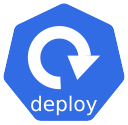
\includegraphics[width=18.66pt,height=18.36pt]{figures/karma_architecture/deploy.png}};
%Image [id:dp5268588430037433] 
\draw (186.74,87.76) node  {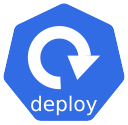
\includegraphics[width=18.66pt,height=18.36pt]{figures/karma_architecture/deploy.png}};
%Image [id:dp7447308292951857] 
\draw (218.44,111.76) node  {
\includegraphics[width=18.66pt,height=18.36pt]{figures/karma_architecture/prometheus.png}};
%Shape: Rectangle [id:dp7837974954754439] 
\draw  [color={rgb, 255:red, 75; green, 101; blue, 225 }  ,draw opacity=1 ][fill={rgb, 255:red, 74; green, 144; blue, 226 }  ,fill opacity=1 ] (202.37,94.64) -- (208.29,94.64) -- (208.29,101.67) -- (202.37,101.67) -- cycle ;
%Shape: Rectangle [id:dp780870970882084] 
\draw  [color={rgb, 255:red, 75; green, 101; blue, 225 }  ,draw opacity=1 ][fill={rgb, 255:red, 74; green, 144; blue, 226 }  ,fill opacity=1 ] (286.37,126) -- (292.29,126) -- (292.29,133.03) -- (286.37,133.03) -- cycle ;

%Shape: Rectangle [id:dp7051683429553395] 
\draw  [color={rgb, 255:red, 75; green, 101; blue, 225 }  ,draw opacity=1 ][fill={rgb, 255:red, 74; green, 144; blue, 226 }  ,fill opacity=1 ] (397.37,124.64) -- (403.29,124.64) -- (403.29,131.67) -- (397.37,131.67) -- cycle ;

%Shape: Rectangle [id:dp5578959475333973] 
\draw  [color={rgb, 255:red, 75; green, 101; blue, 225 }  ,draw opacity=1 ][fill={rgb, 255:red, 74; green, 144; blue, 226 }  ,fill opacity=1 ] (368.37,54.64) -- (374.29,54.64) -- (374.29,61.67) -- (368.37,61.67) -- cycle ;

%Shape: Rectangle [id:dp2822949836407178] 
\draw  [color={rgb, 255:red, 75; green, 101; blue, 225 }  ,draw opacity=1 ][fill={rgb, 255:red, 74; green, 144; blue, 226 }  ,fill opacity=1 ] (324.37,78) -- (330.29,78) -- (330.29,85.03) -- (324.37,85.03) -- cycle ;

%Shape: Rectangle [id:dp9339299822588341] 
\draw  [color={rgb, 255:red, 75; green, 101; blue, 225 }  ,draw opacity=1 ][fill={rgb, 255:red, 74; green, 144; blue, 226 }  ,fill opacity=1 ] (205.37,48) -- (211.29,48) -- (211.29,55.03) -- (205.37,55.03) -- cycle ;



% Text Node
\draw (205.5,98.5) node  [font=\fontsize{0.33em}{0.4em}\selectfont,color={rgb, 255:red, 255; green, 255; blue, 255 }  ,opacity=1 ] [align=left] {1};
% Text Node
\draw (244,58.5) node  [font=\normalsize] [align=left] {{\tiny Scaling}};
\draw (244,64.5) node  [font=\normalsize] [align=left] {{\tiny actions}};
% Text Node
\draw (244,99.5) node  [font=\normalsize] [align=left] {{\tiny Metrics}};
\draw (244,105.5) node  [font=\normalsize] [align=left] {{\tiny data}};
% Text Node
\draw (344.5,36) node  [font=\fontsize{0.33em}{0.4em}\selectfont] [align=left] {\begin{minipage}[lt]{8.66pt}\setlength\topsep{0pt}
\begin{center}
{\fontsize{0.33em}{0.4em}\selectfont $\displaystyle \mathbf{\textcolor[rgb]{0.82,0.01,0.11}{\pi }\textcolor[rgb]{0.82,0.01,0.11}{_{3}}}$}
\end{center}

\end{minipage}};
% Text Node
\draw (341,46.5) node  [font=\fontsize{0.33em}{0.4em}\selectfont] [align=left] {\begin{minipage}[lt]{8.66pt}\setlength\topsep{0pt}
\begin{center}
{\fontsize{0.33em}{0.4em}\selectfont $\displaystyle \mathbf{\textcolor[rgb]{0.82,0.01,0.11}{\pi }\textcolor[rgb]{0.82,0.01,0.11}{_{2}}}$}
\end{center}

\end{minipage}};
% Text Node
\draw (320.9,48) node  [font=\fontsize{0.33em}{0.4em}\selectfont] [align=left] {\begin{minipage}[lt]{8.66pt}\setlength\topsep{0pt}
\begin{center}
{\fontsize{0.33em}{0.4em}\selectfont $\displaystyle \mathbf{\textcolor[rgb]{0.82,0.01,0.11}{\pi }\textcolor[rgb]{0.82,0.01,0.11}{_{1}}}$}
\end{center}

\end{minipage}};
% Text Node
\draw  [color={rgb, 255:red, 75; green, 101; blue, 225 }  ,draw opacity=1 ][fill={rgb, 255:red, 136; green, 197; blue, 246 }  ,fill opacity=1 ][line width=1.5]   (322.77,14.89) .. controls (322.77,13.78) and (323.67,12.89) .. (324.77,12.89) -- (355.77,12.89) .. controls (356.88,12.89) and (357.77,13.78) .. (357.77,14.89) -- (357.77,26.89) .. controls (357.77,27.99) and (356.88,28.89) .. (355.77,28.89) -- (324.77,28.89) .. controls (323.67,28.89) and (322.77,27.99) .. (322.77,26.89) -- cycle  ;
\draw (340.27,20.89) node  [font=\tiny] [align=left] {\begin{minipage}[lt]{21.5pt}\setlength\topsep{0pt}
\begin{center}
KARMA
\end{center}

\end{minipage}};
% Text Node
\draw (290,40.5) node  [font=\tiny] [align=left] {\begin{minipage}[lt]{27.24pt}\setlength\topsep{0pt}
\begin{center}
Organizational\\Analysis
\end{center}

\end{minipage}};
% Text Node
\draw (388,86.39) node  [font=\tiny] [align=left] {\begin{minipage}[lt]{43.42pt}\setlength\topsep{0pt}
\begin{center}
Trained policies
\end{center}

\end{minipage}};
% Text Node
\draw (344.13,127.35) node  [font=\tiny] [align=left] {\begin{minipage}[lt]{60.78pt}\setlength\topsep{0pt}
\begin{center}
PettingZoo environment
\end{center}

\end{minipage}};
% Text Node
\draw (218,127) node  [font=\tiny] [align=left] {\begin{minipage}[lt]{30.31pt}\setlength\topsep{0pt}
\begin{center}
Prometheus
\end{center}

\end{minipage}};
% Text Node
\draw  [color={rgb, 255:red, 75; green, 101; blue, 225 }  ,draw opacity=1 ][fill={rgb, 255:red, 136; green, 197; blue, 246 }  ,fill opacity=1 ][line width=1.5]   (272.9,62) .. controls (272.9,60.9) and (273.8,60) .. (274.9,60) -- (317.9,60) .. controls (319.01,60) and (319.9,60.9) .. (319.9,62) -- (319.9,83) .. controls (319.9,84.1) and (319.01,85) .. (317.9,85) -- (274.9,85) .. controls (273.8,85) and (272.9,84.1) .. (272.9,83) -- cycle  ;
\draw (296.4,72.5) node  [font=\tiny,color={rgb, 255:red, 0; green, 0; blue, 0 }  ,opacity=1 ] [align=left] {Transfer\\Component};
% Text Node
\draw  [color={rgb, 255:red, 75; green, 101; blue, 225 }  ,draw opacity=1 ][fill={rgb, 255:red, 136; green, 197; blue, 246 }  ,fill opacity=1 ][line width=1.5]   (365.88,29.46) .. controls (365.88,28.35) and (366.78,27.46) .. (367.88,27.46) -- (410.88,27.46) .. controls (411.99,27.46) and (412.88,28.35) .. (412.88,29.46) -- (412.88,50.46) .. controls (412.88,51.56) and (411.99,52.46) .. (410.88,52.46) -- (367.88,52.46) .. controls (366.78,52.46) and (365.88,51.56) .. (365.88,50.46) -- cycle  ;
\draw (389.38,39.96) node  [font=\tiny,color={rgb, 255:red, 0; green, 0; blue, 0 }  ,opacity=1 ] [align=left] {Analyzing\\Component};
% Text Node
\draw  [color={rgb, 255:red, 75; green, 101; blue, 225 }  ,draw opacity=1 ][fill={rgb, 255:red, 136; green, 197; blue, 246 }  ,fill opacity=1 ][line width=1.5]   (365.88,98.24) .. controls (365.88,97.13) and (366.78,96.24) .. (367.88,96.24) -- (410.88,96.24) .. controls (411.99,96.24) and (412.88,97.13) .. (412.88,98.24) -- (412.88,119.24) .. controls (412.88,120.34) and (411.99,121.24) .. (410.88,121.24) -- (367.88,121.24) .. controls (366.78,121.24) and (365.88,120.34) .. (365.88,119.24) -- cycle  ;
\draw (389.38,108.74) node  [font=\tiny,color={rgb, 255:red, 0; green, 0; blue, 0 }  ,opacity=1 ] [align=left] {Training\\Component};
% Text Node
\draw (172.5,33.36) node  [font=\tiny] [align=left] {\begin{minipage}[lt]{16.92pt}\setlength\topsep{0pt}
\begin{center}
Cluster
\end{center}

\end{minipage}};
% Text Node
\draw  [color={rgb, 255:red, 75; green, 101; blue, 225 }  ,draw opacity=1 ][fill={rgb, 255:red, 136; green, 197; blue, 246 }  ,fill opacity=1 ][line width=1.5]   (272.9,99) .. controls (272.9,97.9) and (273.8,97) .. (274.9,97) -- (317.9,97) .. controls (319.01,97) and (319.9,97.9) .. (319.9,99) -- (319.9,120) .. controls (319.9,121.1) and (319.01,122) .. (317.9,122) -- (274.9,122) .. controls (273.8,122) and (272.9,121.1) .. (272.9,120) -- cycle  ;
\draw (296.4,109.5) node  [font=\tiny,color={rgb, 255:red, 0; green, 0; blue, 0 }  ,opacity=1 ] [align=left] {Modeling\\Component};
% Text Node
\draw (173,73.72) node  [font=\tiny,rotate=-90] [align=left] {{\LARGE {\fontfamily{helvet}\selectfont \textcolor[rgb]{0.29,0.56,0.89}{...}}}};
% Text Node
\draw (125.61,118.47) node  [font=\tiny] [align=left] {{\LARGE {\fontfamily{helvet}\selectfont \textcolor[rgb]{0.29,0.56,0.89}{...}}}};
% Text Node
\draw (147,89.5) node  [font=\tiny,rotate=-90] [align=left] {{\LARGE {\fontfamily{helvet}\selectfont \textcolor[rgb]{0.29,0.56,0.89}{...}}}};
% Text Node
\draw (125.61,59.9) node  [font=\tiny] [align=left] {{\LARGE {\fontfamily{helvet}\selectfont \textcolor[rgb]{0.29,0.56,0.89}{...}}}};
% Text Node
\draw (208.5,51.86) node  [font=\fontsize{0.33em}{0.4em}\selectfont,color={rgb, 255:red, 255; green, 255; blue, 255 }  ,opacity=1 ] [align=left] {6};
% Text Node
\draw (327.5,81.86) node  [font=\fontsize{0.33em}{0.4em}\selectfont,color={rgb, 255:red, 255; green, 255; blue, 255 }  ,opacity=1 ] [align=left] {5};
% Text Node
\draw (371.5,58.5) node  [font=\fontsize{0.33em}{0.4em}\selectfont,color={rgb, 255:red, 255; green, 255; blue, 255 }  ,opacity=1 ] [align=left] {4};
% Text Node
\draw (400.5,128.5) node  [font=\fontsize{0.33em}{0.4em}\selectfont,color={rgb, 255:red, 255; green, 255; blue, 255 }  ,opacity=1 ] [align=left] {3};
% Text Node
\draw (289.5,129.86) node  [font=\fontsize{0.33em}{0.4em}\selectfont,color={rgb, 255:red, 255; green, 255; blue, 255 }  ,opacity=1 ] [align=left] {2};


\end{tikzpicture}
    \caption{Overview of the KARMA framework in use with a Kubernetes cluster}
    \label{fig:karma_architecture}
\end{figure}

As illustrated in \autoref{fig:karma_architecture}, the KARMA framework operates alongside the Kubernetes cluster, comprising \textbf{worker nodes} that host \textbf{pods}—the atomic unit in Kubernetes containing \textbf{containers} running the actual processes. Pods are organized into \textbf{services} and managed by \textbf{deployments} to update the number of pod refered to as \textbf{replica}. The KARMA framework functions as a separate software layer, interfacing with both the Kubernetes API and Prometheus.

\textbf{1)} Metrics related to availability are gathered as states by \textit{Prometheus}~\cite{prometheus}, a widely adopted time-series metrics database, and processed by KARMA's \textbf{Modeling Component}.

\textbf{2)} Collected states are used to construct a \textit{digital twin} of the cluster as a state transition model. A reward function, defined as a weighted sum of QoS-specific sub-rewards, drives the operational resilience. The digital twin provides a controlled simulation environment to train agents safely without risking disruptions in the real cluster.

\textbf{3)} The \textbf{Training Component} trains agents to maximize rewards to improve operational resilience. Agents are optionally guided by \textit{roles} (constraints shaping their actions) and \textit{missions} (incremental objectives facilitating policy convergence), following the AOMEA methodology~\cite{soule2024aomea}.

\textbf{4)} The \textbf{Analyzing Component} visualize the learned policies through trajectory clustering and hierarchical visualization, ensuring interpretability, alignment with objectives, and resilience to dynamic workloads.

\textbf{5)} The \textbf{Transfer Component} deploys trained policies to the real Kubernetes cluster via the Kubernetes API, executing replica adjustments \textbf{(6)}. Continous interactions between agents and the cluster enables enriching the digital twin with newly collected traces, eventually updating the agents' policy regularly to meet environment's changes.

KARMA integrates simulation-based learning with real-world Kubernetes operations in a closed-loop process. Metrics collected from the cluster guide policy updates, while trained agents' decisions are applied back to the cluster. This iterative process ensures ongoing adaptability, robustness, and resilience under diverse conditions.


\subsection{Modeling}
% Modeling:
%  - observation
%  - actions
%  - rewards -> Faire une récompense qui englobe toutes les QoS ayant pour père la QoS (ne pas faire encore référence aux fonctions de récompense pour l'instant) "availability"
%  - transition -> Transition modeling + MLP -> donner détails des paramètres

In this phase, we assume the initial defender and attacker agents have applied various action in the cluster, leading to a collection of representative amount of traces. Relying on the formalization of the environment as a zero-sum \textbf{Stochastic Game (SG)}~\cite{shapley1953stochastic}, we can provide a near-realistic simulation environment from these collected traces. The SG is characterized by the tuple $\mathcal{SG} = (\mathcal{A}, S, A, T, R, \gamma)$, where $\mathcal{A} = \{\mathcal{A}_d, \mathcal{A}_a\}$ is the agents set comprising $n = |\mathcal{A}_d|$ defender agents and one single attacker agent in $\mathcal{A}_a$; and $\gamma \in [0, 1]$ is the discount factor for future rewards.

\noindent \paragraph{\textbf{State Space}} $S$ is the state space of the Kubernetes cluster. A state denoted as $s \in S$, consists of metrics to characterizing system performance for each of the $d = |D|$ micro-service deployments:
$$
s = (n_{id}, d_{dep}, d_{des}, d_{err}, d_{rem}, r_{cpu}, r_{ram}, t_{in}, t_{out})^d
$$
$n_{id} \in \mathbb{N}$: the deployment number; \quad
$d_{dep} \in \mathbb{N}$: the number of deployed pods; \quad 
$d_{des} \in \mathbb{N}$: the number of desired pods; \quad
$d_{err} \in \mathbb{N}$: the number of failed pods; \quad
$d_{rem} \in \mathbb{N}$: the number of remaining requests to be processed in the queue; \quad
$r_{cpu} \in \mathbb{R}$: the total aggregated CPU (in m) of the pods; \quad
$r_{ram} \in \mathbb{R}$: the total aggregated memory (in Mi) of the pods; \quad
$t_{in} \in \mathbb{R}$: the average received traffic (in Kbps); \quad
$t_{out} \in \mathbb{R}$: the average transmitted traffic (in Kbps).
% TODO: ajouter les métriques spécifiques pour pouvoir vérifier s'il y a des goulots d'étranglement, 

% These metrics are continuously collected using Prometheus~\cite{prometheus}, a widely adopted monitoring and metrics database system, enabling the capture of time-series data for each pod, deployment, and the cluster as a whole.

\noindent \paragraph{\textbf{Action Space}} $A = A_d^n \times A_a$ is the action space with $A_d$ and $A_a$ are the action spaces for a defender and the attacker agents respectively:
$$
a_d \in A_d = (\text{service\_id}, \text{replica\_change})
$$
$\text{\textbf{service\_id}} \in \mathbb{N}$ identifies the target service (through deployment), and $\text{\textbf{replica\_change}} \in [-\alpha, +\alpha]$ indicates the change as for pod replica number (by default $\alpha = 3$). Actions from this space are one-hot encoded as a Box Gym Space~\cite{openAIGymActionSpaces}: for example, the defender actions $(2,1)$, $(0,-2), (1,0)$ mean the services with id numbers equal to $2$, $0$, and $1$ have their respective replica numbers changed by adding $1$, $-2$, $0$.
%
$$
a_a \in A_a = (\text{entry\_point\_id}, \text{rate\_change}, \text{data\_change})
$$
$\text{\textbf{entry\_point\_id}} \in \mathbb{N}$ specifies the service entry point;
$\text{\textbf{rate\_change}} \in \{\text{high\_decrease}, \text{low\_decrease}, \text{no\_change}, \allowbreak \text{low\_increase}, \allowbreak \text{high\_increase}\}$ changes the incoming traffic based on a factor $\kappa$ (by default $\kappa = 1$); and $\text{\textbf{data\_change}} \in \{\text{no\_alteration}, \allowbreak \text{low\_alteration}, \allowbreak \text{high\_alteration}\}$ specifies the degree of data alteration based on factor $\sigma \in [2,\infty[$ (by default $\sigma = 10$). Actions from this space are one-hot encoded as a Box Gym space: for example, the attacker actions $(0,1,2), (2,-1,0), (1,2,1)$ mean that entrypoint services id number 0, 2, and 1 would have their respective traffic-in rates increased by $1 \times \kappa, -1 \times \kappa, 2 \times \kappa$, and respective probabilities to crash due to data alteration are changed by $\frac{2}{\sigma}, \frac{0}{\sigma}, \frac{1}{\sigma}$.

\

\noindent \paragraph{\textbf{Reward Functions}} $R = \{R_d, R_a\}$, with $R_d: S \times A \to \mathbb{R}$ and $R_a: S \times A \to \mathbb{R} = - R_d$ are respectively the reward function for the defender agents based on operational resilience and the attacker one.
To measure operational resilience, we use the linear combination of the following metrics:
%
\begin{itemize}
    \item $\text{Success Rate } (sr) : \frac{\text{Successful Requests}}{\text{Total Received Requests}}$

    \item $\text{Pod Failure Rate } (pfr) : \frac{\text{Failed Pods}}{\text{Total Deployed Pods}}$
    
    \item $\text{Latency Ratio } (lr) : \frac{\text{Measured Latency}}{\text{Maximum Acceptable Latency}}$
    
    \item $\text{Entry Point Availability } (epa) : \frac{\text{Available Entry Points}}{\text{Total Entry Points}}$
    
    \item $\text{Traffic Capacity Ratio } (tcr) : \min\left(1, \frac{\text{Outgoing Traffic}}{\text{Expected Traffic}}\right)$
\end{itemize}
%
$\text{Operational Resilience }: or(s) = w_1 \times sr
\allowbreak + w_2 \times (1 - pfr)
\allowbreak + w_3 \times (1 - lr)
\allowbreak + w_4 \times epa
\allowbreak + w_5 \times tcr
\text{ where } (w_1, w_2, w_3, w_4, w_5) \text{ are relative weights.}$
$$
R_a(s, a_d, a_a) = -R_d(s, a_d, a_a) = or(s)
$$
\text{where $s$ is the current state after applying actions.}

\noindent \paragraph{\textbf{Transition Modeling}} $T: S \times A \rightarrow S = S \times A_d^n \times A_a \to S$ is the real state transition function dictating the next state when the joint actions of the defender agents and the attacker's one are applied. Relying a representative set of collected transitions $\mathcal{T} = \langle(s, a_d^n, a_a, s')_{t\in \mathbb{N}, t \leq w}\rangle$ over a $w$ time window, we can form a partial state transition function $\hat{T}_t$ defined as:
%
$$
\hat{T}_t(s, a_d^n, a_a) =
\begin{cases} 
    s' & \text{if } (s, a_d^n, a_a, s') \in \mathcal{T} \\
    \emptyset & \text{ otherwise}
\end{cases}
$$

To cover no recorded transition, we introduce a Multi-Layer Perceptron (MLP)-based approximator $\hat{T}_a$ to learn from collected transitions and predict the next likely state. The choice of an MLP is motivated by its universal approximation capabilities and the assumption that the next state of a Kubernetes cluster depends only on the current state and the chosen actions.
The MLP approximator has three hidden layers, striking a balance between expressiveness and computational efficiency. The input and output layer dimensions correspond to the size of the state space, while each hidden layer consists of 128 neurons. Rectified Linear Unit (ReLU) activation functions are applied to the hidden layers, and a linear activation function is used at the output layer to produce the predicted next state. The model is optimized using the Adam optimizer with a learning rate of $10^{-3}$, minimizing the Mean Squared Error loss function, expressed as
$$
\mathcal{L} = \frac{1}{N} \sum_{i=1}^N |T(s_i, a_{d,i}, a_{a,i}) - s'_i|^2
$$
where $N$ is a number of representative transitions to ensure generalization.

The complete modeled transition function $\hat{T}$ is defined as:
$$
\hat{T}(s, a_d, a_a) = 
\begin{cases} 
\hat{T}_t(s, a_d, a_a) & \text{if } (s, a_d, a_a) \in \text{Domain}(\hat{T}_t), \\
\hat{T}_a(s, a_d, a_a) & \text{otherwise}.
\end{cases}
$$

\noindent \paragraph{\textbf{Digital Twin Environment}} The defined action and state space with approximated transition function $\hat{T}$, combined with the reward functions $R_d$ and $R_a$, forms the basis of the digital twin environment implemented using the PettingZoo library~\cite{Terry2021}. This environment enables simulating the Kubernetes cluster from the defined SG, enabling safe exploration of defender agents against different attacker strategies.



\subsection{Training}
\label{sec:training}

In this phase, MARL algorithms are applied within the modeled environment to enable agents to learn and maximize cumulative rewards. As suggested in AOMEA~\cite{soule2024aomea}, we leverage the $\mathcal{M}OISE^+$ organizational model to bring ways to control/guide the MARL training. In the KARMA framework it results in a decomposition of the overarching goal of \textit{operational resilience} into sub-objectives. Each sub-objective is assigned to a specific agent as a mission, while roles define rule-based strategies to guide agent operations.\\

\noindent \textbf{Agent Roles and Missions}

A \textbf{role} is formally represented by a \textbf{Role Action Guide} (RAG), which restricts an agent's permissible actions:
$$
rag(h, \omega) = (\{a_1, a_2, \dots, a_i\}, ch)
$$
where $h$ represents the trajectory or history, \(\omega\) is the agent's observation, and \(ch \in \{0,1\}\) is the constraint hardness, set to 1 by default. A hard constraint (\(ch = 1\)) strictly limits the agent's available actions to authorized ones, while a soft constraint (\(ch = 0\)) allows for exploratory actions but adjusts rewards with bonuses or penalties based on compliance with the authorized action set. For example, the \textbf{Bottleneck Resolution Agent} has a role restricting its actions to modifying pod replicas within a specific service graph, ensuring it does not affect unrelated services. If a bottleneck is detected in Service A that causes delays in Service B, the agent adheres to its role by increasing the pod replicas of Service A to resolve the issue without overstepping constraints.

A \textbf{mission} is a set of intermediate goals designed to assist in achieving the overarching operational resilience objective. Missions are represented by a \textbf{Goal Reward Guide} (GRG), which incentivizes mission completion:
$$
grg(h) = r_b,
$$
where \(h \in H\) represents the current agent trajectory and \(r_b \in \mathbb{R}\) is the associated reward bonus or penalty. This mechanism narrows the optimization focus to critical resilience tasks. For instance, the \textbf{DDoS Detector and Responde} is assigned a mission to maintain service availability during Distributed Denial-of-Service (DDoS) attacks. It earns a reward bonus for ensuring that a predefined percentage of incoming requests is successfully handled, despite the increased load, by dynamically adjusting replicas. The mission aligns the agent's focus on balancing load while avoiding resource over-provisioning.\\

By defining specific \textbf{(role, mission)} pairs, the KARMA framework assigns specialized tasks to agents to tackle distinct challenges in chained Kubernetes services. These roles and missions enable distributed yet coordinated policy learning, ensuring that agents align their actions to maximize overall \textit{operational resilience}. For example, while the Bottleneck Resolution Agent alleviates bottlenecks to ensure steady service throughput, its actions complement those of the DDoS Detector and Responder, which adjusts replicas to mitigate traffic surges. This interdependence highlights the importance of coordinating roles and missions to address shared challenges.

\paragraph*{Algorithms and training pipeline}

\

KARMA integrates MADDPG~\cite{lowe2017multi} (Multi-Agent Deep Deterministic Policy Gradient), which is well-suited to stabilize policy updates and enable effective inter-agent communication~\cite{lowe2017multi}, ensuring coordination on strategies. Communication is critical in KARMA due to the interdependencies between agent roles and missions, such as how Bottleneck Detector can influence adversarial response priorities.

The training pipeline in KARMA follows a systematic sequence to optimize agent behaviors. Initially, policies (\(\pi_i\)), roles (RAG), and missions (GRG) are defined for all agents to establish a structured framework. Agents participate in simulation runs, generating trajectories within the digital twin environment. At each step, roles with hard constraints restrict the available actions to authorized ones, while soft constraints influence rewards by applying bonuses or penalties based on compliance. Missions add further reward shaping by incentivizing goal-aligned trajectories. The \textit{Optuna}~\cite{akiba2019optuna} framework is used for Hyper-Parameter Optimization, iteratively refining policies by adjusting hyperparameters and role specifications to improve convergence and enhance system resilience.

Convergence is deemed successful when the standard deviation of cumulative rewards across episodes falls below a predefined threshold $\mu \in \mathbb{R}$, and cumulative rewards exceed an empirically determined minimum value $\sigma \in \mathbb{R}$.


\subsection{Analysis}
\label{sec:analysis}

The analysis phase in the KARMA framework aims to validate and interpret the behaviors of trained agents, ensuring their alignment with operational objectives and their robustness in dynamic or adversarial environments. \textbf{Explainability} is essential for verifying that agents' collective behaviors align with system objectives and for building trust with human operators~\cite{biran2017explanation, guidotti2018survey}. While each agent in KARMA has a defined role and mission, the complexity arises when agents must coordinate in dynamic scenarios, such as:
\begin{itemize}
    \item \textbf{Normal conditions}, where all agents act independently without risking conflicts.
    \item \textbf{Critical conditions}, requiring rapid intervention and prioritization of specific agents.
    \item \textbf{Adversarial conditions}, such as Distributed DDoS attacks, where coordination must prevent conflicting or redundant actions.
\end{itemize}

For example, during a DDoS attack, an agent may take precedence to ensuring that the other agents' actions are not uselessly applied. This necessitates understanding how agents implicitly or explicitly negotiate priorities and coordinate~\cite{Shoham2008}.

\paragraph*{\textbf{Inferring Roles and Missions}}

To enhance the explainability of agent behaviors, roles and missions can be derived from the trajectories of trained agents using data-driven methods:

\begin{itemize}
    \item \textbf{Role Generation}:
\end{itemize}

\noindent Hierarchical clustering identifies recurring sequences of actions that define an agent's role. The distance between action sequences is computed using Dynamic Time Warping~\cite{berndt1994using} (DTW) for analyzing the sequences of agents' actions taking into account variations in timing across the different test episodes:
\[
d(\tau_i, \tau_j) = \min_{\pi} \sum_{k=1}^{|\pi|} \|a_{t_k}^i - a_{t_k}^j\|_2,
\]
where $\pi$ is the optimal alignment path. Clustering hyperparameters, such as the number of clusters, are empirically tuned to minimize noise and avoid generating spurious roles. Clusters are annotated to define abstract roles, such as "Bottleneck Detector" or "DDoS Detector and Responder"

\begin{itemize}
    \item \textbf{Mission Generation}:
\end{itemize}    

\noindent K-means clustering groups trajectories based on similarity in states visited. The cluster centers represent common objectives, and recurrent observations in high-reward trajectories are sampled to define intermediate goals:
    \[
    g_i = \mathcal{S}_j, \quad \text{where } \mathcal{S}_j = \{s \in \tau_i | \mathbb{P}(s) > \epsilon\}.
    \]
    Here, $\mathbb{P}(s)$ represents the probability of visiting a state $s$ within successful trajectories. $\epsilon$ represents a threshold used to filter states $s$ based on their probability $\mathbb{P}(s)$ of being visited to minimize noise. Hyperparameters of K-means are empirically optimized to minimize noise.


\paragraph*{\textbf{Detecting Inter-Agent Interactions}}

Explainability in KARMA also requires an understanding of how agents coordinate their actions in different contexts. This is achieved by analyzing inter-agent relationships using the concepts of \textbf{MOISE+}, which formalizes relations such as acquaintance, authority, and communication~\cite{hubner2002moise}:
\begin{itemize}
    \item \textbf{Acquaintance Relations}: Derived from shared observations or reward signals during training, these relations represent which agents are aware of each other's actions.
    \item \textbf{Authority Relations}: Captured through dependency patterns, authority relations prioritize one agent's decisions over another's in specific scenarios. For instance, an specific agent may hold authority during a DDoS attack.
    \item \textbf{Communication Relations}: Inferred from synchronized actions or information-sharing events. For example, agents sharing traffic load data to coordinate replica adjustments during surges.
\end{itemize}

To visualize these relations, a directed graph can be constructed where nodes represent agents and edges represent relations, annotated with interaction type on a time window.
%Considering a time window, we can generate a graph based on detected relations and may evolves dynamically on the next time window, highlighting changes in interaction patterns.

% In addition, we also determine the \textbf{patterns of coordination} that aim to understand the mutual impact of an agent's actions onto another agent's trajectory  over time. Among Sequential Pattern Mining, we favoured the use of the \textit{PrefixSpan} algorithm to identify recurring action sequences across agents during specific scenarios. For example, patterns may show that one agent defers actions to another during adversarial conditions. Detected sequences can be represented as a sequence diagram illustrates how agents interact over time, showing causal relationships and dependencies in resolving challenges.



\subsection{Transfer}
\label{sec:transfer}

% Transfering: Processus de transfert des comportements appris au cluster réel.
%  - récupérer les politiques entrainés dans un sous-module
%  - lancer les politiques entrainés avec l'état courant collecté
%  - appliquer les actions choisies par ces politiques via l'API K8s

The final phase in the KARMA framework deploys trained and validated agent policies into the live Kubernetes cluster operating as a continuous loop:
\begin{enumerate}
    \item \textbf{State Collection:} Real-time metrics such as CPU usage, memory consumption, pod status, and network traffic are collected from the Prometheus server~\cite{prometheus}.
    \item \textbf{Policy Execution:} Each agent's policy $\pi_i$ computes an action $a_t^i$ based on the current state $s_t$, selecting adjustments such as scaling pod replicas for a deployment.
    \item \textbf{Action Application:} The computed actions are sent as API requests, directly modifying deployment.
\end{enumerate}
This loop ensures agents continuously respond to changes in workload and system conditions.
%
% The agents interact seamlessly with Kubernetes:
% \begin{enumerate*}[label={}, itemjoin={;\quad }]
%     \item Actions are applied to deployments via the API
%     \item Real-time metrics are gathered using Prometheus, ensuring up-to-date cluster state observations
%     \item KARMA operates independently of the native Kubernetes HPA mechanisms.
% \end{enumerate*}

% \

% \noindent The framework integrates a feedback loop:
% \begin{enumerate*}[label=\textbf{\arabic*)}, itemjoin={;\quad }]
%     \item Metrics from the live cluster are used to update the digital twin model.
%     \item Agents are periodically retrained on this updated model to refine their policies for new workload patterns or adversarial conditions.
%     \item Refined policies are redeployed to the cluster, maintaining high adaptability and resilience.
% \end{enumerate*}



% =======================================
\section{Experimental Setup}
\label{sec:experiments}
% Experimental setup:
%  - Présenter "Chained Services"
%  - CybMASDE: présenter comme un moyen d'implémenter KARMA et présenter la configuration logicielle
%  - Configuration matérielle (pour entrainement et analyse)
%  - Protocole d'experimentation et d'analyse (prend en compte un espèce d'étude d'ablation dans les baselines)
%  - Métriques d'évaluation
%  - Baselines: MA x (Org. Spec.)
%     - modèle sans specifications organisationnelles avec 1 seul agent (état de l'art)
%     - modèle avec spécifications organisationnelles du modèle "fort" avec 1 seul agent (état de l'art?)
%     - modèle sans spécifications organisationnelles avec plusieurs agents (état de l'art?)
%     - modèle avec spécifications organisationnelles du modèle "faible" avec plusieurs agents
%     - modèle avec spécifications organisationnelles du modèle "fort" avec plusieurs agents

This section outlines the experimental setup for evaluating KARMA's ability to address initially defined gaps.

\subsection{Description of the Kubernetes Cluster and Configuration}

The evaluation environment consists of a Kubernetes cluster simulating a \textbf{Chained Services} (CS) architecture. Each service comprises a set of microservices hosted in pods and managed by deployments. For instance, \autoref{fig:chained_services_graph} illustrates the graph representation of a four services CS cluster. We considered using a cluster characterized by the following specifications:

\begin{itemize}
    \item \textbf{Topology:} 20 interconnected running services configured to emulate real-world conditions, including resource contention, bottlenecks, and adversarial scenarios;
    \item \textbf{Failure Simulation:} Bottlenecks and cascading failures are induced by resource-intensive workloads, while adversarial conditions (e.g., DDoS attacks) are emulated using Locust~\cite{locust2021} and random-based custom scripts;
    \item \textbf{Worker Nodes:} 1 worker node with 8 vCPUs, 32 GB RAM, and 1 Gbps network bandwidth. This configuration is suitable for testing purposes on medium-sized clusters;
    \item \textbf{Training Node:} 1 high computing cluster comprising nodes with NVIDIA Tesla V100 GPUs (16GB), Intel Xeon Platinum CPUs (2.3 GHz, 16 cores), 128 GB RAM.
\end{itemize}

\begin{figure}[h!]
    \centering
    \hspace{-0.4cm}
    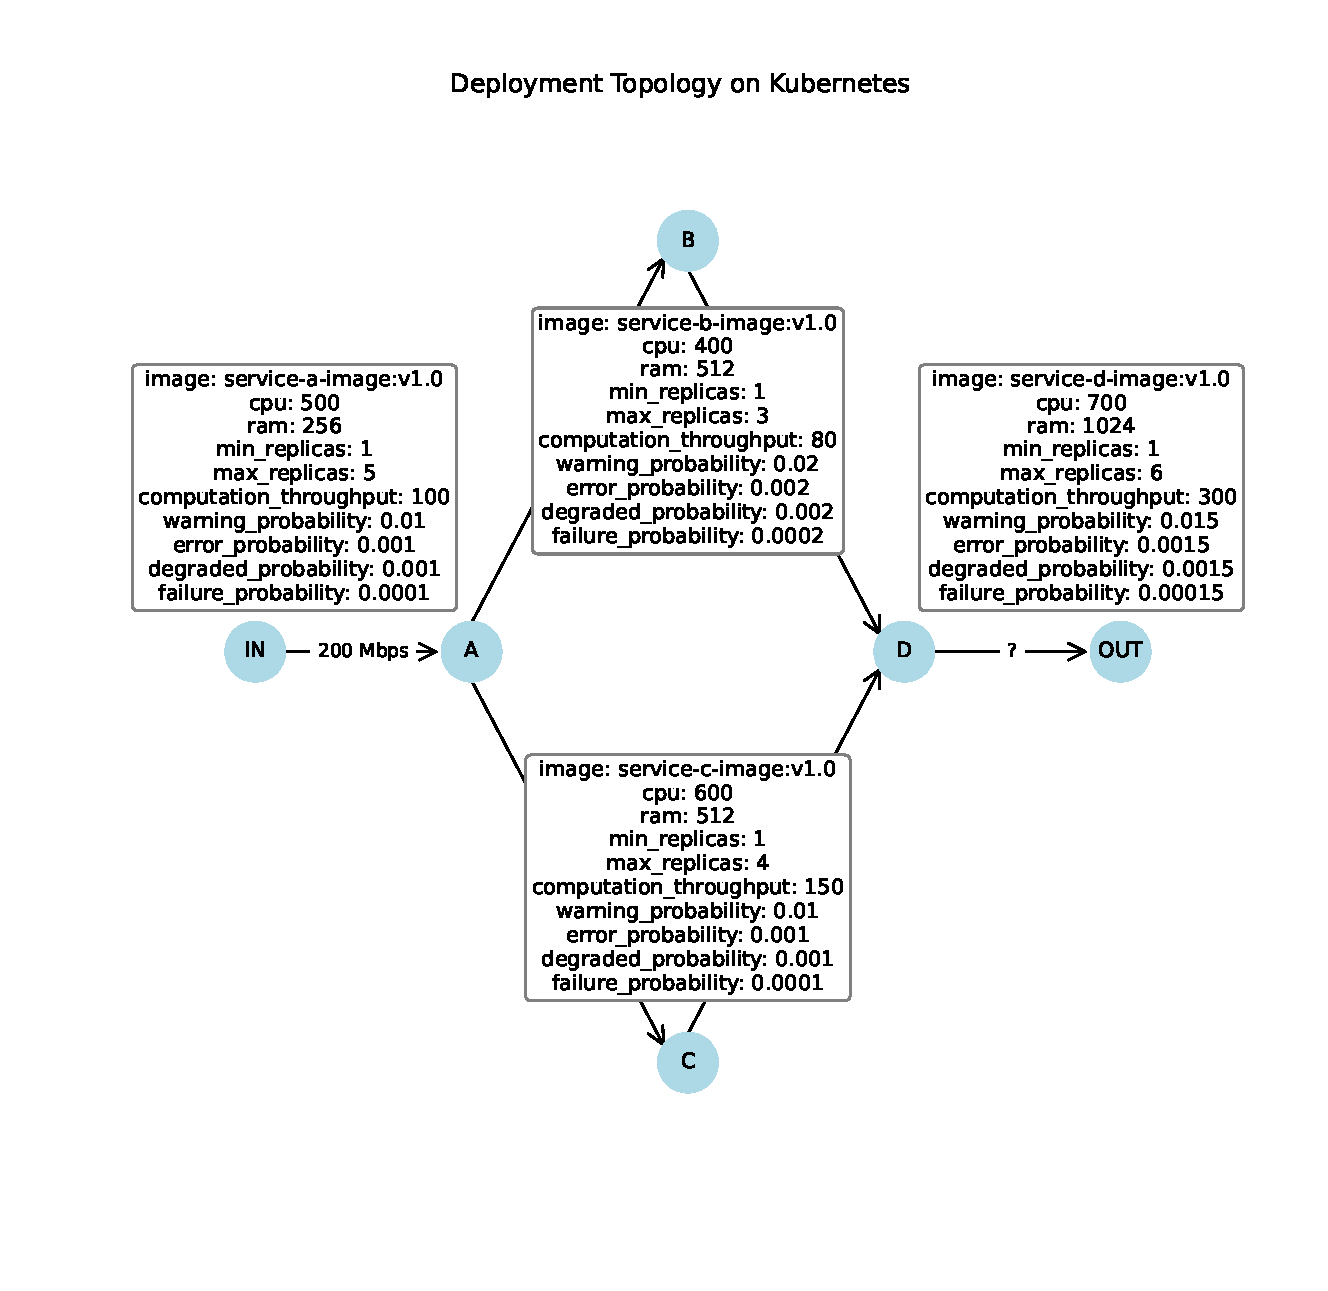
\includegraphics[trim=1.8cm 3.3cm 1.25cm 3.5cm, clip, width=0.5\textwidth]{figures/k8s_cluster_graph.pdf}
    \caption{A graph representation of a "Chained Services" cluster with four services}
    \label{fig:chained_services_graph}
\end{figure}

\subsection{Implementation of KARMA with CybMASDE}

% TODO:
% - Présenter le framework CybMASDE
% - Scénario normal, scénario DDoS (augmentation ponctuelle de volume données), scénario de défaillance (corruption ponctuelle des données), scénario de contention de ressources (priorisation), scénario mixte
% - Protocole d'expérimentation
%   - Baseline 1: Single-Agent w/o Soft Organizational Specifications
%   - Baseline 2: Single-Agent w/ Hard Organizational Specifications
%   - Baseline 3: Multi-Agent w/o Organizational Specifications
%   - Baseline 4: Multi-Agent w/ Organizational Specifications

The KARMA framework leverages \textit{Cyber Multi-Agent System Development Environment}~\footnote{Source code available with extra details
% and Jupyter Notebook
at: \url{https://anonymous.4open.science/r/KARMA-040B/README.md}} (CybMASDE) that is a general assisted-design MAS fitting in which the KARMA framework is developed. The framework includes:
\begin{itemize}
    \item \textbf{Digital Twin Modeling:} A simulation environment replicates Kubernetes cluster using real-world traces.
    \item \textbf{MARL Training:} \textit{MADDPG}~\cite{lowe2017multi} is used to train agents in the digital twin environment.
    \item \textbf{Organizational Specifications:} Roles and missions defined for agents guide the training process, ensuring coordinated behavior and explainability.
    \item \textbf{Deployment Integration:} Trained policies interact with the Kubernetes API to adjust pod replicas in real time.
\end{itemize}

\subsection{Roles and Missions for Operational Resilience}

\noindent Following to the $\mathcal{M}OISE^+$~\cite{hubner2002moise} and the AICA architectural insights~\cite{kott2018autonomous}, we implemented four roles to address a specific degradation factor in a QoS.
% and defines the permissible actions of agents.
Each role is associated with a mission, containing a single sub-objective based on metrics.

\noindent \paragraph{\textbf{Bottleneck Detector}} 
%
The \textit{Bottleneck Detector} role is to monitor services for bottlenecks caused by imbalanced traffic flows. It is based on rules following these metrics:
\begin{enumerate*}[label={}, itemjoin={;\quad }]
    \item \( T_{\text{in}}^i \): Incoming traffic for service \( i \) (Kbps)
    \item \( T_{\text{out}}^i \): Outgoing traffic for service \( i \)
    \item \( Q_{\text{pending}}^i \): Pending requests for service \( i \).
\end{enumerate*}
A bottleneck is detected if: $Q_{\text{pending}}^i > Q_{\text{threshold}} \quad \text{or} \quad T_{\text{in}}^i > \alpha \cdot T_{\text{out}}^i$
where \( Q_{\text{threshold}} \) is the critical queue threshold, and \( \alpha > 1 \) is an amplification factor.

The associated mission aims to minimize the pending queue size to eliminate bottlenecks. The reward function is defined as: $R_{\text{bottleneck}} = - \sum_{i} Q_{\text{pending}}^i$
Agents are rewarded for reducing pending requests, optimizing the throughput~\cite{burns2016borg}.

\noindent \paragraph{\textbf{DDoS Detector and Responder}}

The \textit{DDoS Detector} role is to identify DDoS attacks by analyzing traffic anomalies:
\begin{enumerate*}[label={}, itemjoin={;\quad }]
    \item \( R_{\text{rate}} \): Incoming request rate for the cluster.
    \item \( L_{\text{avg}} \): Average observed latency.
    \item \( \Delta T \): Change in traffic volume over a time window \( t \).
\end{enumerate*}
A DDoS attack is detected when:
$R_{\text{rate}} > R_{\text{threshold}} \quad \text{and} \quad \Delta T > \Delta T_{\text{threshold}}$
where \( R_{\text{threshold}} \) is a critical traffic threshold.

The associated mission is to isolate affected services to minimize downtime with this reward function:
$R_{\text{ddos}} = - \left( \text{DownTime} \cdot w_{\text{d}} + L_{\text{avg}} \cdot w_{\text{l}} \right)$
where \( w_{\text{d}} \) and \( w_{\text{l}} \) are weights for downtime and latency, respectively~\cite{koller2019ddos}.

\noindent \paragraph{\textbf{Failure Manager}}

The \textit{Failure Manager} role is to monitor pod health and eliminates failed pods following this rule:
\begin{enumerate*}[label={}, itemjoin={;\quad }]
    \item \( F_{\text{fail}}^i \): Number of failures for pod \( i \).
    \item \( S_{\text{status}}^i \): Status of pod \( i \) (e.g., \textit{CrashLoopBackOff}).
\end{enumerate*}
A pod failure is detected if:
$F_{\text{fail}}^i > F_{\text{threshold}}$
where \( F_{\text{threshold}} \) is the maximum number of tolerated failures.

The associated mission minimizes downtime caused by repeated failures with this reward function:
$R_{\text{failure}} = - \sum_{i} T_{\text{downtime}}^i$
Agents are incentivized to quickly eliminate and restart failed services.

\noindent \paragraph{\textbf{Resource Allocator}}

The \textit{Resource Allocator} role is to prioritize critical services when resource contention occurs. The rules are based on:
\begin{enumerate*}[label={}, itemjoin={;\quad }]
    \item \( U_{\text{cpu}}^i \): CPU utilization of service \( i \).
    \item \( U_{\text{mem}}^i \): Memory utilization of service \( i \).
    \item \( P_{\text{priority}}^i \): Priority level of service \( i \) (critical, normal, low).
\end{enumerate*}
Contention is detected if total CPU usage exceeds a threshold:
$U_{\text{cpu}}^{\text{total}} > U_{\text{threshold}}$
Non-critical services are scaled down to free resources:
$\text{Replicas}_{\text{new}}^i = \max\left( \text{Replicas}_{\text{current}}^i - \delta, 1 \right)$

The associated mission ensures critical services by balancing resource usage with this reward function:
$R_{\text{resource}} = - \sum_{i \in \text{Critical}} \left( U_{\text{cpu}}^i + U_{\text{mem}}^i \right)$
Agents are rewarded for prioritizing services while maintaining efficient resource usage~\cite{smith2021autoscaling}.

\

\subsection{Experimental Protocol}

\noindent To evaluate the performance of KARMA in addressing the six identified gaps, we propose comparing baselines assessed through the same scenarios.

\paragraph{\textbf{Experimental Scenarios}}

\noindent Five experimental scenarios are defined to simulate key factors impacting operational resilience in Kubernetes:

\begin{itemize}
    \item \textbf{Bottleneck Resolution:} Simulates scenarios where upstream services overload downstream services to maximize throughput by dynamically scaling replicas.
    \item \textbf{DDoS Attack:} Models a sudden surge in traffic aimed at disrupting critical services to detect the attack, isolate affected services, and minimize downtime~\cite{koller2019ddos}.
    \item \textbf{Pod Failures:} Pod crashes are triggered to evaluate the system's ability to restore affected services~\cite{burns2016borg}.
    \item \textbf{Resource Contention:} Simulates high resource demand, requiring dynamic prioritization of critical services to maintain overall cluster functionality~\cite{zhang2020resource}.
    \item \textbf{Mixed Scenario:} Combines all scenarios to evaluate the system's adaptability and resilience.
\end{itemize}

\paragraph{\textbf{Baselines from the literature}}

\noindent We selected three HPA systems as baselines for comparison:
\begin{itemize}
    \item \textbf{AWARE:} An RL-based system that balances response time and throughput~\cite{aware2023}.
    \item \textbf{Gym-HPA:} An RL environment for experimentation with various RL algorithms in simulation~\cite{gym_hpa}.
    \item \textbf{IMAM:} A multi-agent framework that incorporates RL but lacks organizational constraints~\cite{imam2022}.
\end{itemize}

These baselines have been tested under the same five scenarios using source code when available.

\paragraph{\textbf{Baselines as ablation studies}}

\noindent To isolate the contributions of KARMA's components, ablation studies have been performed following these configurations:
\begin{itemize}
    \item \textbf{With/without MLP:} Evaluates the impact of using an MLP-based transitioner for digital-twin modeling.
    \item \textbf{With/without organizational specifications:} Tests hard and soft organizational constraints during training:
        \begin{itemize}
            \item \textit{Hard constraints:} Strictly enforce roles and missions.
            \item \textit{Soft constraints:} Allow exploratory actions with rewards based on organizational specifications.
        \end{itemize}
    \item \textbf{Multi-agent vs Mono-agent:} Compares a multi-agent configuration with a mono-agent baseline.
\end{itemize}

\paragraph{\textbf{Performance Metrics}}

\noindent For each scenario and baseline, the following metrics are collected:

\begin{itemize}
    \item \textbf{Operational Resilience:} Based on the global reward from the success rate (\%), ratio of pending request (\%), average latency (ms)~\cite{burns2016borg}.
    \item \textbf{Adversarial Robustness:} Based on the standard deviation of the reward and the recovery time after DDoS (s), percentage of services remaining available (\%)~\cite{koller2019ddos}.
    \item \textbf{Digital Twin Accuracy:} Based on the modeled transition model accuracy (\%), computed as the ratio of real cluster performance over the simulation's one~\cite{moreno2018kubernetes}.
    \item \textbf{Automated MAS Generation:} Based on training convergence time (number of episodes)~\cite{smith2021autoscaling}.
    \item \textbf{Adaptability:} Based on the reward standard deviation variance over training episodes on all scenarios (\%)~\cite{aware2023}.
    \item \textbf{Explainability:} Based on alignment of behaviors with roles/missions when given (\%), and qualitative evaluation of clustering of trajectories (dendrogram) otherwise~\cite{hubner2002moise}.
\end{itemize}

% \paragraph{\textbf{Analysis and Comparison}}

% \begin{enumerate}
%     \item \textbf{Baseline Comparisons:} Compare KARMA's performance to the state-of-the-art baselines across all metrics and scenarios.
%     \item \textbf{Gap Validation:} Verify that KARMA addresses the gaps effectively by demonstrating superior performance on associated metrics.
%     \item \textbf{Ablation Studies:} Analyze the impact of removing key components (MLP, organizational specifications, etc.) to quantify their contributions.
% \end{enumerate}

% \paragraph{Expected Outcome.} KARMA is expected to outperform existing baselines in operational resilience, adversarial robustness, adaptability, and explainability, while demonstrating the unique advantages of its digital twin modeling and automated MAS generation.


\section{Results and Discussion}
\label{sec:results}

This section analyzes the performance of KARMA in addressing the six identified gaps.

\subsection{Gap 1: Operational Resilience}
Operational resilience evaluates the ability of the system to handle failures and maintain high QoS. Metrics such as success rate, latency compliance, and pending requests ratio were analyzed across all scenarios. Table~\ref{tab:operational_resilience} presents a comparison of KARMA against most baselines.
%
\begin{table}[h]
    \centering
    \caption{Operational resilience metrics across all scenarios.}
    \label{tab:operational_resilience}
    \begin{tabular}{>{\raggedright\arraybackslash}m{2.7cm}>{\centering\arraybackslash}m{1.5cm}>{\centering\arraybackslash}m{1.5cm}>{\centering\arraybackslash}m{1.5cm}}
        \hline
        \textbf{Baseline} & \textbf{Success Rate (\%)} & \textbf{Latency Compliance (\%)} & \textbf{Pending Requests (\%)} \\
        \hline
        KHPA & 65.4 & 58.7 & 21.3 \\
        Gym-HPA & 70.8 & 63.4 & 18.5 \\
        IMAM & 76.2 & 68.9 & 14.7 \\
        AWARE & 80.1 & 73.3 & 12.8 \\
        \textit{Single-Agent w/o Org. Spec.} & 74.3 & 67.1 & 18.7 \\
        \textit{Single-Agent w/ Hard Org. Spec.} & 83.9 & 75.6 & 12.3 \\
        \textit{Multi-Agent w/o Org. Spec.} & 86.5 & 79.2 & 10.5 \\
        \textit{Multi-Agent w/ Soft Org. Spec.} & 90.3 & 84.1 & 6.7 \\
        \textbf{Multi-Agent w/ Hard Org. Spec. (KARMA)} & \textbf{93.7} & \textbf{88.5} & \textbf{3.1} \\
        \hline
    \end{tabular}
\end{table}

KARMA achieves the highest success rate (93.7\%) and latency compliance (88.5\%), while minimizing pending requests to just 3.1\%, significantly outperforming all baselines. In the \textit{Bottleneck Resolution} scenario, KARMA effectively reduces pending requests to 2.8\%, enabling higher throughput compared to AWARE (12.3\%). In the \textit{Resource Contention} scenario, KARMA prioritizes critical services, achieving a latency compliance of 90.3\%, compared to 82.1\% for IMAM.

KHPA struggles with dynamic workloads due to its reactive, threshold-based rules, resulting in lower success rates and higher pending requests. AWARE and IMAM provide moderate improvements but lack the explicit multi-agent coordination and organizational constraints of KARMA. The addition of organizational specifications in KARMA ensures well-aligned actions among agents, reducing latency and maximizing QoS across diverse conditions.

\subsection{Gap 2: Adversarial Conditions}
Adversarial conditions evaluate the system's robustness against disruptive scenarios such as Distributed Denial-of-Service (DDoS) attacks. Metrics include recovery time and service availability across all scenarios. Table~\ref{tab:adversarial_conditions} compares KARMA's performance to other baselines.

\begin{table}[h]
    \centering
    \caption{Performance under adversarial conditions (DDoS scenario).}
    \label{tab:adversarial_conditions}
    \begin{tabular}{>{\raggedright\arraybackslash}m{3.6cm}>{\centering\arraybackslash}m{1.8cm}>{\centering\arraybackslash}m{2cm}}
        \hline
        \textbf{Baseline} & \textbf{Recovery Time (s)} & \textbf{Service Availability (\%)} \\
        \hline
        KHPA & 82.4 & 67.3 \\
        Gym-HPA & 68.1 & 74.5 \\
        IMAM & 55.3 & 80.2 \\
        AWARE & 50.7 & 84.8 \\
        \textit{Single-Agent w/o Org. Spec.} & 60.2 & 72.3 \\
        \textit{Single-Agent w/ Hard Org. Spec.} & 45.3 & 80.7 \\
        \textit{Multi-Agent w/o Org. Spec.} & 40.1 & 85.4 \\
        \textit{Multi-Agent w/ Soft Org. Spec.} & 35.2 & 89.6 \\
        \textbf{Multi-Agent w/ Hard Org. Spec. (KARMA)} & \textbf{28.5} & \textbf{95.2} \\
        \hline
    \end{tabular}
\end{table}

KARMA consistently achieves the best performance in the DDoS scenario. As for \textit{Recovery Time}, KARMA recovers 28.9\% faster than Multi-Agent w/o Org. Spec. (40.1 s), demonstrating effective collaborative agent coordination. The \textit{Service Availability} with KARMA is about 95.2\%, showing it maintains higher availability compared to AWARE (84.8\%) and KHPA (67.3\%).

Baselines like KHPA and Gym-HPA struggle to adapt to sustained adversarial loads, leading to slower recovery times and reduced service availability.
KARMA's hard organizational specifications enable agents to prioritize critical actions and minimize conflicting responses, ensuring faster recovery and greater availability during attacks.

\subsection{Gap 3: Digital Twin Modeling}
The accuracy of the digital twin model is critical for training agents under realistic conditions. This evaluation focuses on the transition model's accuracy in simulating Kubernetes dynamics across all scenarios. Table~\ref{tab:digital_twin_accuracy} summarizes the results.

\begin{table}[h]
    \centering
    \caption{Digital twin transition model accuracy across all scenarios.}
    \label{tab:digital_twin_accuracy}
    \begin{tabular}{>{\raggedright\arraybackslash}m{6cm}>{\centering\arraybackslash}m{2cm}}
        \hline
        \textbf{Baseline} & \textbf{Accuracy (\%)} \\
        \hline
        Without MLP Transition Model & 85.3 \\
        With MLP Transition Model (KARMA) & \textbf{94.8} \\
        \hline
    \end{tabular}
\end{table}

KARMA's MLP-based transition model achieves a higher accuracy (94.8\%) compared to the baseline (85.3\%). The inclusion of an MLP approximator enhances the digital twin's ability to generalize across scenarios by capturing complex state transitions. This improvement is particularly evident in the \textit{Resource Contention} scenario, where accurate modeling of resource bottlenecks ensures effective policy training.

Without an MLP, the transition model struggles to generalize, leading to suboptimal agent behaviors in dynamic environments. The high accuracy achieved by KARMA's model enables agents to better anticipate system responses, improving their ability to handle unforeseen workload patterns. This result underscores the importance of integrating machine learning-based approximators in simulation environments for realistic multi-agent reinforcement learning scenarios.


\subsection{Gap 4: Automated MAS Generation}

The efficiency of generating a Multi-Agent System (MAS) is evaluated in terms of convergence time and training overhead. Table~\ref{tab:mas_generation_efficiency} presents the results across all scenarios while \autoref{fig:learning_curves} shows learning curves for the main baselines in the mixed scenario over 2000 episodes.

\begin{table}[h]
    \centering
    \caption{MAS generation efficiency across all scenarios.}
    \label{tab:mas_generation_efficiency}
    \begin{tabular}{>{\raggedright\arraybackslash}m{3.5cm}>{\centering\arraybackslash}m{2cm}>{\centering\arraybackslash}m{2cm}}
        \hline
        \textbf{Baseline} & \textbf{Convergence Time (episodes)} & \textbf{Training Overhead (hours)} \\
        \hline
        Multi-Agent w/o Org. Spec. & 1800 & 4 \\
        \textbf{Multi-Agent w/ Hard Org. Spec. (KARMA)} & \textbf{950} & \textbf{1.5} \\
        \hline
    \end{tabular}
\end{table}

As for \textit{Convergence Time} KARMA reduces convergence time by roughly 50\% compared to the baseline without organizational specifications. Additionally, the process requires about 35\% less \textit{Training Overhead} with KARMA, due to restricted policy search space and contributing to enhance scalability.

The role-guided learning narrows the search space for optimal policies, enabling faster convergence and reduced computational costs. These efficiency gains are particularly important for scaling MAS solutions to complex environments.

\begin{figure}[h!]
    \centering
    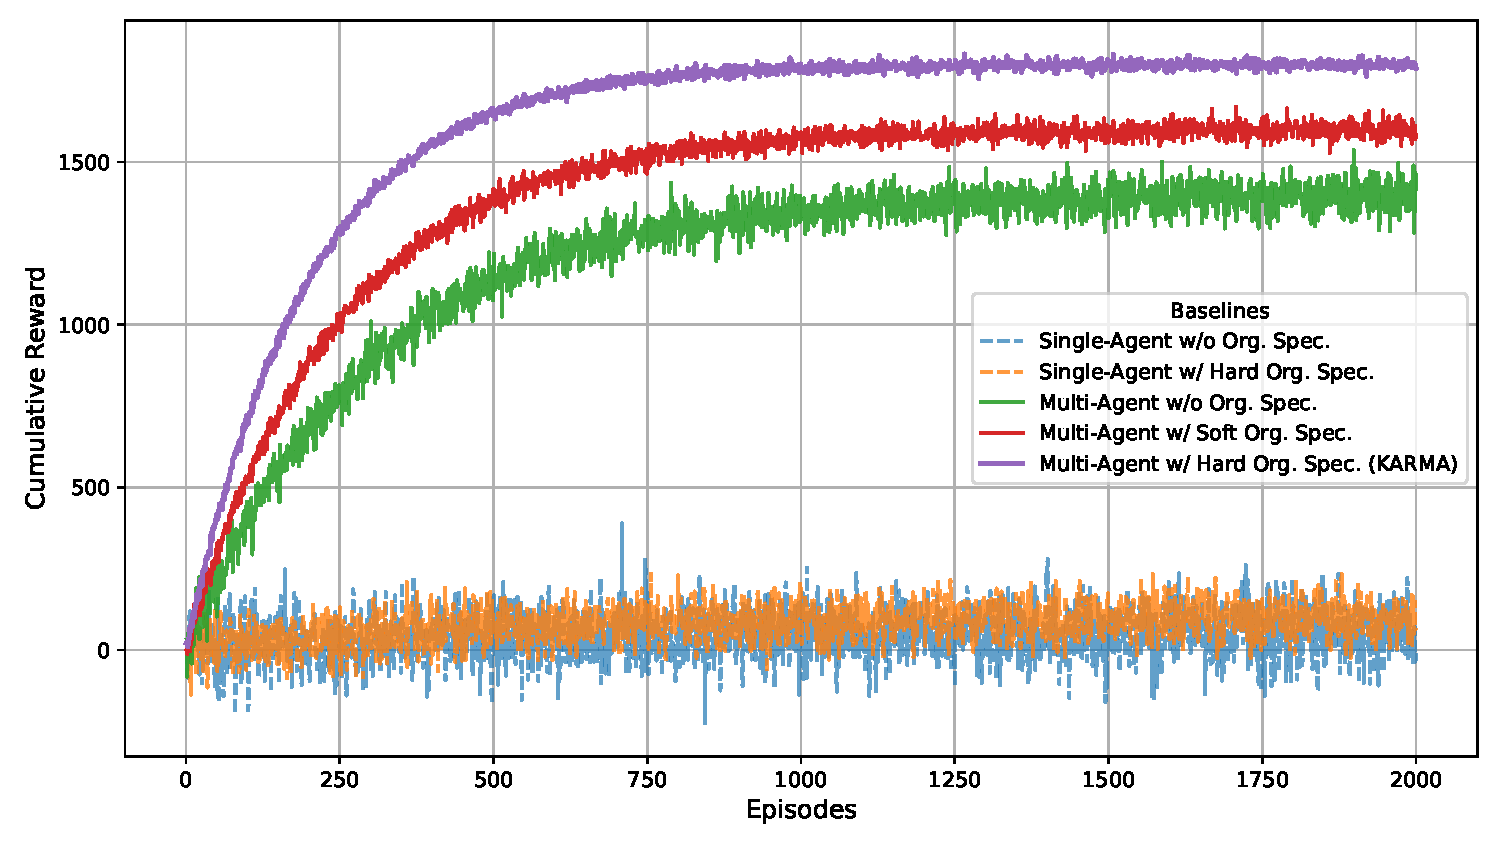
\includegraphics[width=0.49\textwidth]{figures/learning_curves.pdf}
    \caption{Learning curves across baselines for the mixed scenario over 2000 episodes.}
    \label{fig:learning_curves}
\end{figure}


\subsection{Gap 5: Adaptability}
Adaptability assesses the ability of the system to maintain performance under dynamic workloads and heterogeneous conditions. The reward standard deviation in the mixed scenario was measured and presented in Table~\ref{tab:adaptability_comparison}.

\begin{table}[h]
    \centering
    \caption{Comparison of adaptability metrics in the mixed scenario.}
    \label{tab:adaptability_comparison}
    \begin{tabular}{>{\raggedright\arraybackslash}m{5cm}>{\centering\arraybackslash}m{3cm}}
        \hline
        \textbf{Baseline} & \textbf{Reward Variance (\%)} \\
        \hline
        Single-Agent w/o Org. Spec. & 12.4 \\
        Single-Agent w/ Hard Org. Spec. & 8.9 \\
        Multi-Agent w/o Org. Spec. & 7.3 \\
        \textbf{Multi-Agent w/ Hard Org. Spec. (KARMA)} & \textbf{3.1} \\
        \hline
    \end{tabular}
\end{table}

In the \textit{Mixed Scenario}, KARMA maintains stable performance across dynamically changing workloads, outperforming the next-best baseline (7.3\% variance). KARMA shows resilience against abrupt workload shifts with consistent rewards.

Organizational constraints provide agents with clear priorities, reducing conflicting actions and ensuring stability and allow distributed decision-making, which enhances responsiveness to dynamic conditions. The reduced reward variance underscores KARMA’s ability to generalize across diverse scenarios, making it well-suited for real-world deployments.

\subsection{Gap 6: Explainability}
\label{subsec:gap_explainability}

Explainability is qualitatively evaluated through trajectory clustering and quantitatively through the alignment of agent behaviors with predefined roles and missions.
\noindent \autoref{fig:trajectory_clustering_hrl} illustrates the dendrogram generated by hierarchical clustering of agents' action sequences with the four roles applied, using DTW as the similarity measure. The figure highlights the emergence of four distinct clusters, each corresponding to a specific organizational role, demonstrating the ability of the agents' behaviors to align with the predefined roles.

\begin{figure}[h!]
    \centering
    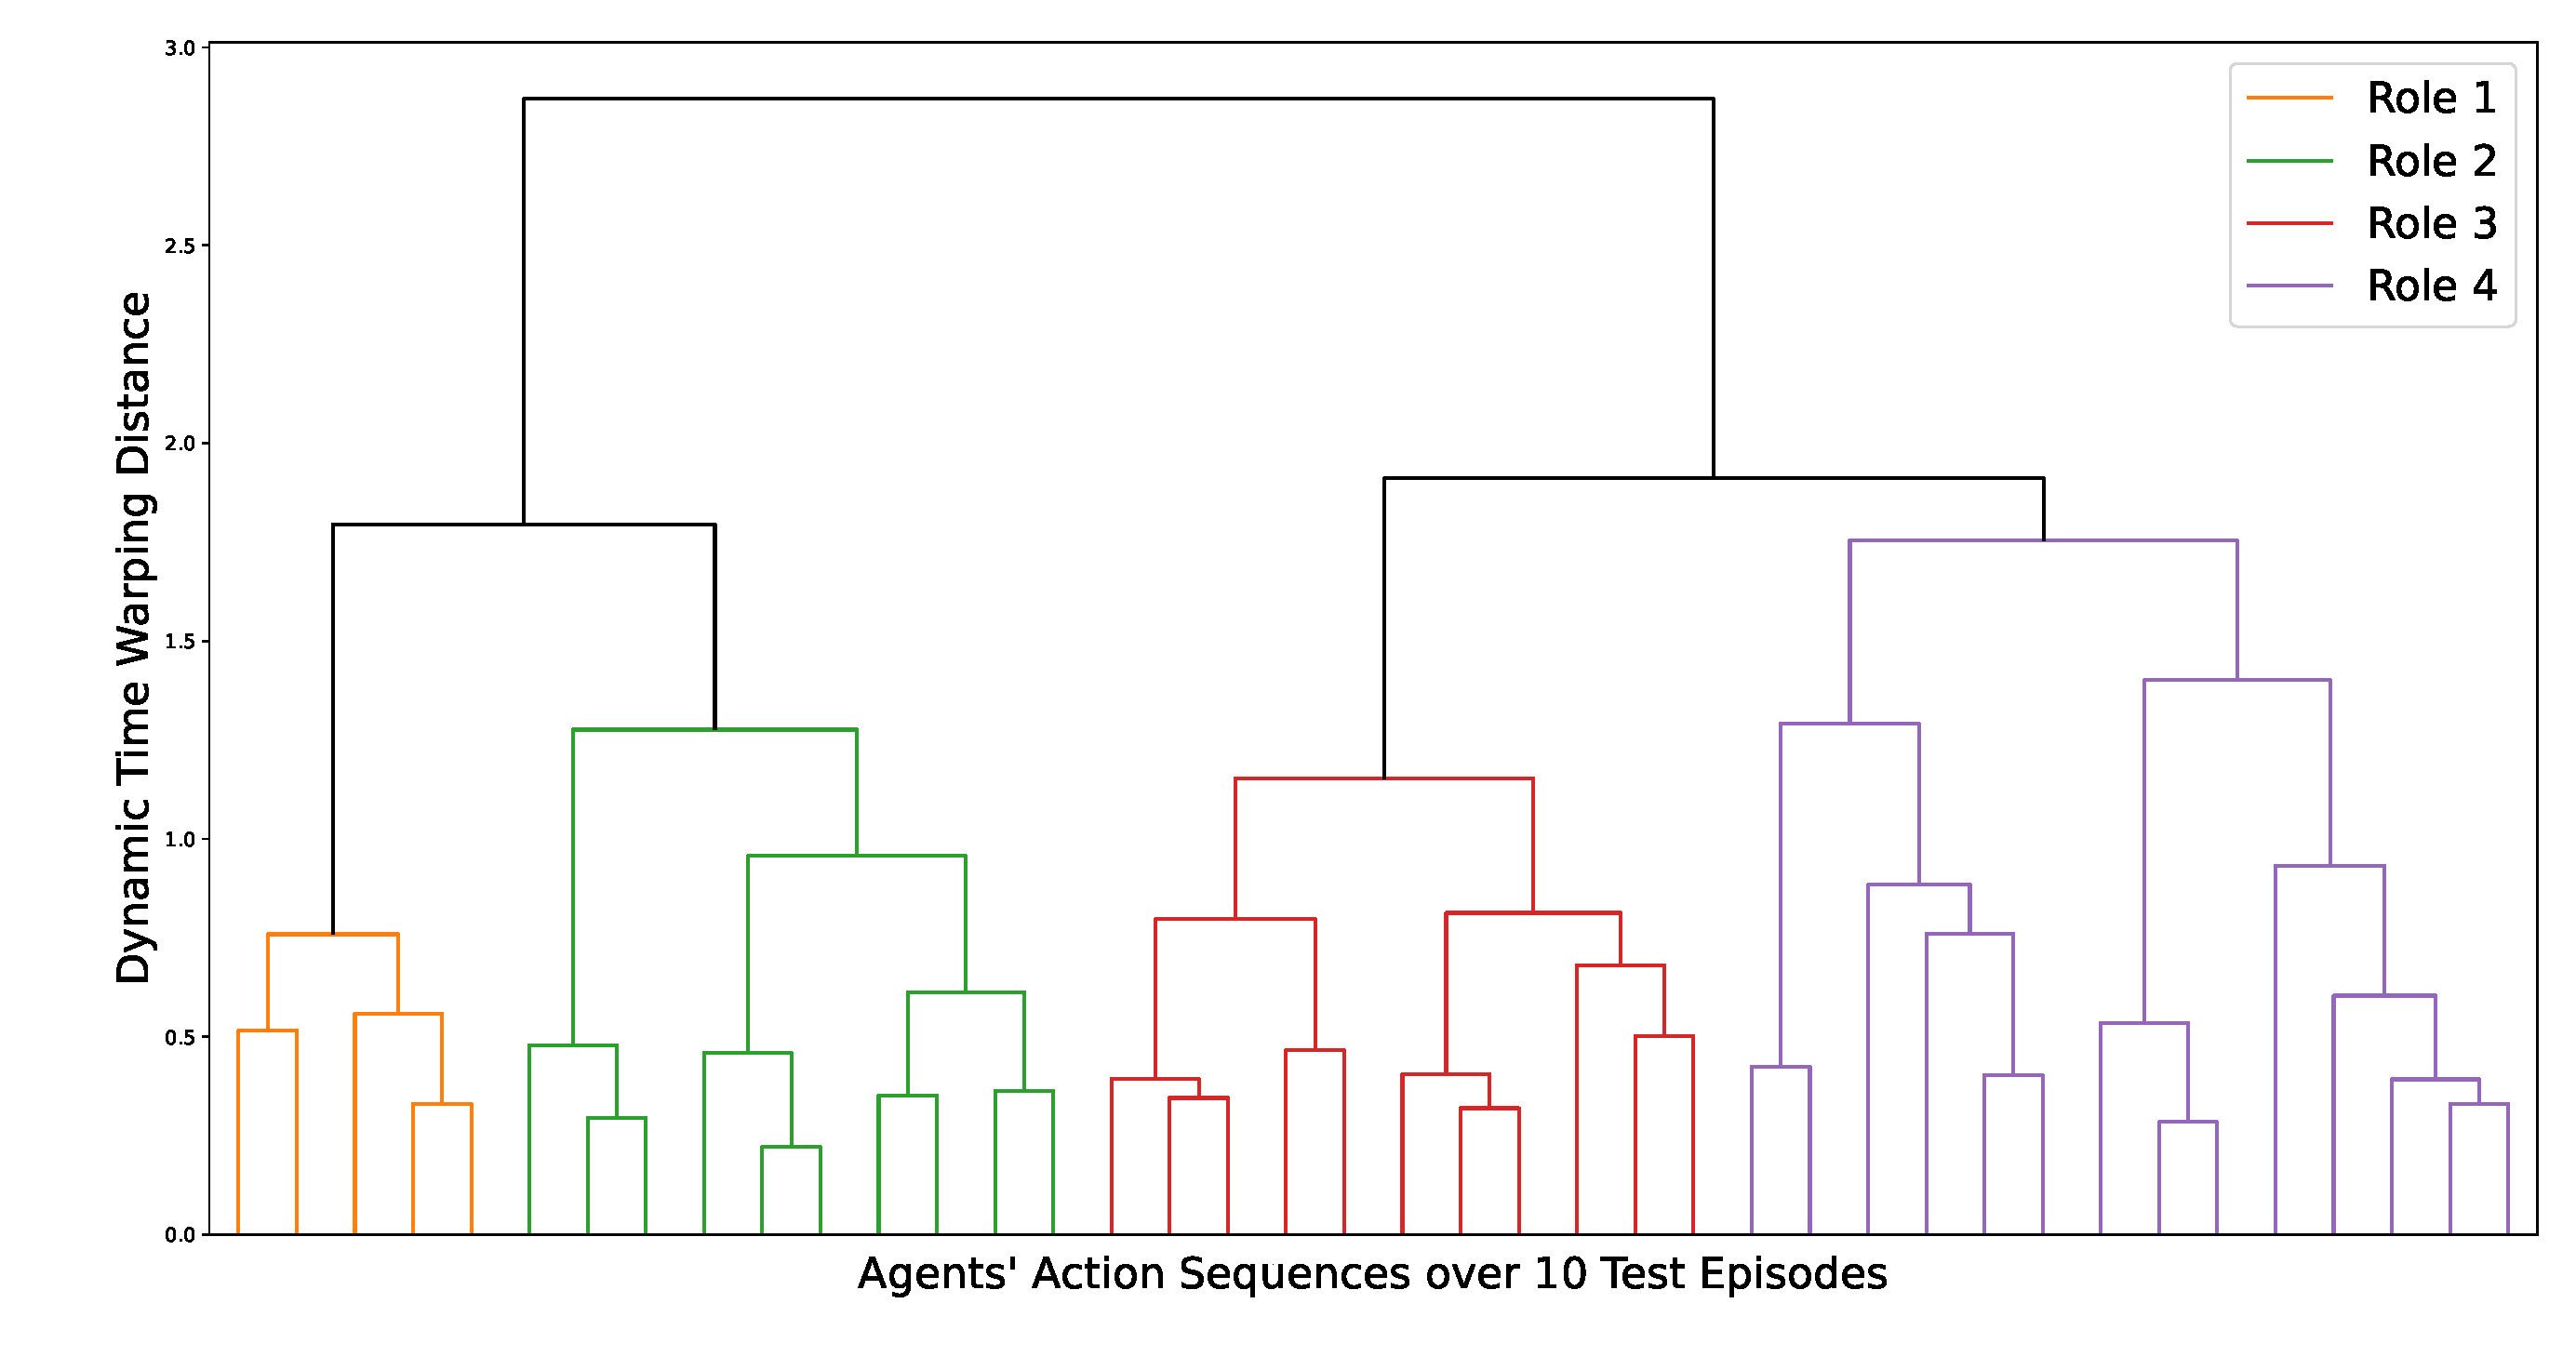
\includegraphics[width=0.49\textwidth]{figures/role_hierarchical_clustering.pdf}
    \caption{Dendrogram obtained after hierarchical clustering of agent trajectories for role inference in the mixed scenario.}
    \label{fig:trajectory_clustering_hrl}
\end{figure}

\begin{table}[h!]
    \centering
    \caption{Alignment of Agent Behavior with Roles and Missions.}
    \label{tab:alignment}
    {\scriptsize
    \begin{tabular}{>{\raggedright\arraybackslash}m{3.5cm}>{\centering\arraybackslash}m{2cm}>
    {\centering\arraybackslash}m{2cm}}
    \toprule
    \textbf{Baseline} & \textbf{Alignment Score (\%)} & \textbf{Clustering Purity (\%)} \\
    \midrule
    Multi-Agent w/o Org. Spec. & $\emptyset$ & 62.7 \\
    Multi-Agent w/ Soft Org. Spec. & 85.3 & 70.1 \\
    Multi-Agent w/ Hard Org. Spec. (KARMA) & \textbf{96.2} & \textbf{89.4} \\
    \bottomrule
    \end{tabular}
    }
\end{table}

KARMA shows the emergence of distinct behavioral patterns aligned with predefined roles validates KARMA's organizational model and has the highest alignment score (96.2\%), significantly outperforming Multi-Agent w/o Org. Spec. (78.5\%), showcasing well-coordinated agent behaviors. In adversarial scenarios, clustering purity is highest for KARMA, reflecting the clear differentiation of agent behaviors under organizational constraints.

Distinct clusters validate the role-specific behaviors and highlight the interpretability of agent policies. Baselines without organizational specifications show reduced explainability, as evidenced by lower clustering purity and alignment scores with soft constraints for organizational specifications.

% \subsection{General discussion}

% The experimental results demonstrate that KARMA effectively addresses several critical gaps in Kubernetes autoscaling. By integrating MARL with organizational principles, KARMA achieves notable improvements in operational resilience, adversarial robustness, and explainability. Its ability to decompose complex objectives into roles and missions ensures coordinated agent behavior, as reflected in the high success rates, reduced recovery times, and alignment with predefined roles observed across all scenarios. The use of a digital twin environment, enhanced by an MLP-based transition model, further strengthens KARMA's capacity to simulate realistic conditions, facilitating robust training and better policy generalization.

% However, KARMA is not without limitations. While it shows advancements in adaptability, its dependence on domain expertise for defining roles and missions could limit its applicability in domains where such expertise is scarce. Additionally, the computational overhead required for multi-agent training and digital twin modeling remains a challenge for large-scale deployments. The results also indicate that while KARMA effectively reduces latency and pending requests, some baselines, such as IMAM, perform comparably in specific scenarios like resource contention, highlighting areas where further refinement may be needed.

\section{Conclusion}
\label{sec:conclusion}
% Conclusion
%  - Résumé
%  - Résumé des Points faibles et Perspectives

This paper presented KARMA, a framework aimed at improving the operational resilience of Kubernetes clusters through a MAS-based approach.
The experimental results demonstrate that KARMA effectively addresses several critical gaps in Kubernetes autoscaling. By integrating MARL with organizational principles, KARMA achieves improvements in adversarial robustness, and explainability. Its ability to decompose complex objectives into roles and missions ensures coordinated agent behavior, as reflected in the high success rates, reduced recovery times. The use of MLP-based transition model, further strengthens KARMA's capacity to simulate realistic conditions, facilitating better policy generalization.
%
% The main contributions of this work include:
% \begin{itemize}
%     \item \textbf{Digital Twin Environment:} A realistic and representative simulation model derived from cluster traces, enabling safe and efficient policy learning through a digital twin.
%     \item \textbf{Organizationally Guided Design:} The use of roles and missions to decompose operational resilience into manageable sub-objectives, providing a systematic method for agent coordination and decision-making.
%     \item \textbf{Multi-Agent Reinforcement Learning (MARL):} Leveraging MARL algorithms to train agents collaboratively, ensuring adaptability and robustness in complex, multi-objective scenarios.
%     \item \textbf{Explainability and Analysis:} Analyzing agent behaviors using trajectory clustering and inter-agent interaction detection, enhancing interpretability and trust in agent decisions.
%     \item \textbf{Adversarial Scenario Handling:} Demonstrating the resilience of the proposed framework in scenarios such as DDoS attacks, which are critical for the reliability of cloud-native systems.
% \end{itemize}
%
% \

However, some aspects need to be further explored:
\begin{enumerate*}[label=\textbf{\arabic*)}, itemjoin={;\quad }]
    \item \textbf{Dependence on Domain Expertise:} Defining roles, missions, and reward structures relies heavily on domain-specific knowledge, which may limit the framework's generalizability to other domains.
    \item \textbf{Computational Overhead:} The training process, particularly with multi-agent configurations and organizational constraints, requires substantial computational resources, posing challenges for large-scale clusters.
    % \item \textbf{Sensitivity to Workload Shifts:} While KARMA demonstrates adaptability, abrupt changes in workload patterns or cluster configurations may require retraining or fine-tuning of agent policies.
    % \item \textbf{Evaluation Scope:} Although the framework was tested under diverse scenarios, including adversarial conditions, its performance on larger and more heterogeneous clusters remains to be validated.
\end{enumerate*}

Building on these initial results, several future research directions can be pursued to enhance KARMA's capabilities:
\begin{itemize}
    \item \textbf{Automated Role and Mission Generation:} Leveraging data-driven methods or pre-trained knowledge bases to automatically define roles and missions, reducing the reliance on domain expertise.
    % \item \textbf{Efficient Training Pipelines:} Exploring optimization techniques, such as transfer learning or distributed training, to mitigate the computational overhead of multi-agent training.
    \item \textbf{Dynamic Role Adjustment:} Investigating mechanisms for agents to dynamically adapt their roles and missions, enhancing flexibility and responsiveness.
    \item \textbf{Generalization to Larger Clusters:} Extending the framework to more complex, large-scale Kubernetes deployments with heterogeneous configurations.
    % \item \textbf{Integration with Real-Time Monitoring:} Incorporating advanced monitoring systems to further refine the digital twin model and provide more accurate state representations.
\end{itemize}

% While KARMA is not a universal solution to all Kubernetes autoscaling challenges, it provides a step forward in addressing key gaps in operational resilience, adaptability, and explainability. The framework's combination of MARL and organizational principles offers a promising foundation for future research and development.

\section*{Acknowledgment}
    This work was supported by \emph{Thales Land Air Systems} within the framework of the \emph{Cyb'Air} chair and the \emph{AICA IWG}.

\section*{References}

\nocite{alDhuraibi2017elasticDocker}

% \bibliographystyle{abbrv}
\bibliographystyle{IEEEtran}

\bibliography{references}

\end{document}
